%%%--- Template for master thesis at SfS
%%%--- Modified template with more comments and examples -- SG, 11/06/09
%%%------
\documentclass[11pt,a4paper,twoside,openright]{report}
\usepackage[english]{ETHDAsfs}%--> ETHDASA + fancyhdr + ... "umlaute"
%  + sfs-hyper -> hyperref 

\usepackage{pdfpages}%%to include the confirmation of originality (plagiarism
\usepackage{amsbsy}%% for \boldsymbol and \pmb{.}
\usepackage{amssymb}%% calls  amsfonts...
\usepackage{graphicx}%-- für PostScript-Grafiken (besser als  psfig!)
%\usepackage[draft]{graphicx} % grafics shown as boxes --> faster compilation
%
\usepackage[longnamesfirst]{natbib}%was {sfsbib}%- Für  Literatur-Referenzen
%           ^^^^^^^^^^^^^^ 1) "Hampel, Ronchetti, ..,"  2) "Hampel et al"
% Engineers (and other funny people) want to see [1], [2] 
% ---> use 'numbers' : \usepackage[longnamesfirst,number]{natbib}
%
%
\usepackage{texab}%- 'tex Abkürzungen' /u/sfs/tex/tex/latex/texab.sty
        %%- z.B.  \R, \Z, \Q, \Nat für reelle, ganze, rationale, natürl. Zahlen;
        %%-       \N   (Normalvert.)  \W == Wahrscheinlichkeit .....
        %%-  \med, \var, \Cov, \....
        %%-  \abs{x} == |x|   und   \norm{y} ==  || y ||   (aber anständig)
%% NOTE: texab contains many useful definitions and "shortcuts". It is
%% worth to open the file and have a look at them. HOWEVER, some
%% definitions are a bit can lead to conflicts with other packages. You
%% might for example want to comment out the line defininf \IF as an
%% operator when working with the algorithmic package, or to comment out
%% the line defining a command \Cite with working with the Biblatex package  
\usepackage{amsmath,amsfonts,mathtools}
%\usepackage{mathrsfs}% Raph Smith's Formal Script font --> provides \mathscr
\usepackage[utf8]{inputenc}% <<------- Unicode, *NOT* iso-latin1 !
\usepackage{url}
\usepackage{ae}% A[lmost] E[uropean] Fonts
\usepackage{enumerate}% Fuer selbstdefinierte Nummerierungen
%--------
\usepackage{relsize}%-> \smaller (etc) used here
\usepackage{color} %% to allow coloring in code listings
\usepackage{listings}% Fuer R-code, C-code, ....  and settings for these:
\definecolor{Mygrey}{gray}{0.75}% for linenumbers only!
\definecolor{Cgrey}{gray}{0.4}% for comments
\lstloadlanguages{R}

%%--- first version of "listings of R"-style : ---------------------------
% %% using \smaller here: makes R code listings use a *small* font:
% \lstset{language=R,basicstyle=\smaller[2],commentstyle=\rmfamily\smaller,
%   showstringspaces=false,xleftmargin=4ex,
%   literate={<-}{{$\leftarrow$}}1 {~}{{$\sim$}}1}
% \lstset{escapeinside={(*}{*)}} % for (*\ref{ }*) inside lstlistings (Scode) 
%\newcommand{\lil}[1]{\lstinline|#1|}
%%--- newer version of "listings of R"-style : ---------------------------
\lstset{%% Help, e.g. --> https://en.wikibooks.org/wiki/LaTeX/Source_Code_Listings
language=R,
basicstyle=\ttfamily\scriptsize,%%- \small > \footnotesize > \scriptsize > \tiny
%commentstyle=\ttfamily\color{Cgrey},
commentstyle=\itshape\color{Cgrey},
numbers=left,
numberstyle=\ttfamily\color{Mygrey}\tiny,
stepnumber=1,
numbersep=5pt,
backgroundcolor=\color{white},
showspaces=false,
showstringspaces=false,
showtabs=false,
frame=single,
tabsize=2,
captionpos=b,
breaklines=true,
%breakatwhitespace=false,
keywordstyle={},
morekeywords={},
xleftmargin=4ex, 
literate={<-}{{$\leftarrow$}}1 {~}{{$\sim$}}1}
\lstset{escapeinside={(*}{*)}} % for (*\ref{ }*) inside lstlistings (Scode) 
%%----------------------------------------------------------------------------

%%------- Theoreme ---
\newtheorem{definition}{Definition}[subsection]
\newtheorem{lemma}[definition]{Lemma}
\newtheorem{theorem}[definition]{Theorem}
\newtheorem{Coro}[definition]{Corollary}
\theoremstyle{definition} 
\newtheorem{example}[definition]{Example}
\newtheorem*{note}{Note}
\newtheorem*{remark}{Remark}

\DeclareMathOperator*{\plim}{plim}
% \def\MR#1{\href{http://www.ams.org/mathscinet-getitem?mr=#1}{MR#1}}

% \newcommand{\Lecture}[3]{\marginpar{#3.#2.#1}}
% \newcommand{\Fu}{\mathcal{F}}
\newcommand{\aatop}[2]{\genfrac{}{}{0pt}{}{#1}{#2}}

%\renewcommand{\theequation}{\arabic{equation}}
\numberwithin{equation}{subsection}

%%%%%%%%%%%%%%%%%%%%%%%%%%%%%%%%%%%%%%%%%%%%%%%%%
%%% Path for your figures                      %%%
%%%%%%%%%%%%%%%%%%%%%%%%%%%%%%%%%%%%%%%%%%%%%%%%%
% Set the paths where all figures are taken from:
\graphicspath{{Pictures/}}

%%%%%%%%%%%%%%%%%%%%%%%%%%%%%%%%%%%%%%%%%%%%%%%%%
%%% Define your own commands here             %%%
%%%%%%%%%%%%%%%%%%%%%%%%%%%%%%%%%%%%%%%%%%%%%%%%%
\newcommand{\Bruch}[2]{{}^{#1}\!\!/\!_{#2}}
\renewcommand{\labelenumi}{\roman{enumi}.)}

% \usepackage{chngcntr}
\counterwithout{equation}{subsection}
\counterwithout{equation}{chapter}

\begin{document}
\bibliographystyle{chicago}% ---> Hampel,F., E.Ronchetti,... W.Stahel(1986) ...
 %was \bibliographystyle{sfsbib}\citationstyle{dcu} %OR DEFAULT : \citationstyle{agsm}

\pagenumbering{roman}%- roman numbering for first few pages

%%%%%%%%%%%%%%%%%%%%%%%%%%%%%%%%%%%%%%%%%%%%%%%%%
%%% Title page                                %%%
%%%%%%%%%%%%%%%%%%%%%%%%%%%%%%%%%%%%%%%%%%%%%%%%%
\period{Spring 2024}
\dasatype{Master Thesis}
\students{Yiting Nian}
\mainreaderprefix{Advisor:}
\mainreader{Dr. Fabio Sigrist}
\alternatereaderprefix{}
% \alternatereader{Your co-supervisor}
\submissiondate{June 14, 2024}
\title{Optimization methods for Gaussian process hyper-parameter estimation}

\maketitle%- Titelseite wird abgeschlossen
\cleardoublepage
 %%~~~~~~~~~~~~~~~~~~~~~~~~~~~~~~~~~~~~~~~~

%%%%%%%%%%%%%%%%%%%%%%%%%%%%%%%%%%%%%%%%%%%%%%%%%
%%% Insert here acknowledgements and abstract %%%
%%%%%%%%%%%%%%%%%%%%%%%%%%%%%%%%%%%%%%%%%%%%%%%%%
%% Dedication (optional)
% \markright{}
% \vspace*{\stretch{1}}
% \begin{center}
%     To some special person
% \end{center}
% \vspace*{\stretch{2}}

% Preface (optional)
\newpage
\markboth{Preface}{Preface}
% \chapter*{Preface}

First words and acknowledgements.

%%% Local Variables: 
%%% mode: latex
%%% TeX-master: "MasterThesisSfS"
%%% End: 


% Abstract should not be longer than one page.
\newpage
\markboth{Abstract}{Abstract}
\chapter*{Abstract}

Gaussian process (GP) is a flexible statistical and machine learning model that is widely used in applications involving time series or spatial data. To make predictions based on this model, several hyper-parameters in the covariance function have to be estimated. In this thesis, we perform a systematic comparison of several commonly used optimization methods, which based on gradients, secondary derivatives, or heuristic search strategy, for the estimation of Gaussian process hyper-parameters from the perspective of training speed, convergence performance, pros and cons. Approximation methods are used for the large spatial data to reduce the computation burden. Simulated data samples of different settings and distributions will be used to test the performance of the optimization methods, then theoretical and experimental comparison will be summarized. %Afterwards, application suggestions will be summarized. 

%%% Local Variables: 
%%% mode: latex
%%% TeX-master: "MasterThesisSfS"
%%% End: 


%%%%%%%%%%%%%%%%%%%%%%%%%%%%%%%%%%%%%%%%%%%%%%%%%
%%% Table of contents and list of figures and %%%   
%%% tables (no need to change this usually)   %%%
%%%%%%%%%%%%%%%%%%%%%%%%%%%%%%%%%%%%%%%%%%%%%%%%%
\newpage
\tableofcontents
\newpage
\listoffigures
\newpage
\listoftables

%% Notations and glossary (optional)
\cleardoublepage
\phantomsection
\addcontentsline{toc}{chapter}{\protect\numberline{}{Notation}}
\markboth{Notation}{Notation}
\chapter*{Notation}
\label{c:Notation}

%Explain your symbols and abbreviations.
GP - Gaussian process

GD - Gradient Descent

BFGS - Broyden–Fletcher–Goldfarb–Shanno

LBFGS -  Limited-memory BFGS

FITC - Fully Independent Training Conditional


%%% Local Variables: 
%%% mode: latex
%%% TeX-master: "MasterThesisSfS"
%%% End: 


\cleardoublepage
\pagenumbering{arabic}%--- switch back to standard numbering 


%%%%%%%%%%%%%%%%%%%%%%%%%%%%%%%%%%%%%%%%%%%%%%%%%
%%% Your text... Either write here directly,  %%%
%%% or even better: write in separate files   %%%
%%% that you just have to include here.       %%% 
%%%%%%%%%%%%%%%%%%%%%%%%%%%%%%%%%%%%%%%%%%%%%%%%%
\chapter{Introduction} 

% Description of the work. Prepare the reader for the following chapters.

% You will cite literature here, typically, but

Gaussian process (GP) regression, or kriging (\cite{eidsvik2011spatial}), is a popular non-parametric function model that combines the characteristics of easy-implementing, flexibility, and modelling accuracy. Gaussian Processes (GPs) have applications in various areas, such as non-parametric regression, time series or spatial data, and emulation of large computer models (\cite{kennedy2001bayesian}). The defining features of a GP are its mean function and covariance function (kernel), which are parameterised by different variables; depending on different classes of covariance function. Hyper-parameters in GPs include parameters of the covariance function, the noise variance and, in some cases, parameters of the mean function. The covariance function, which defines the similarity between data points, is particularly sensitive and crucial; as it directly affects the smoothness and overall shape of the predicted function. In this thesis, we focus on the Mat\'ern class of covariance functions (\cite{williams2006gaussian}). 

The practical utility of GPs largely depends on the accurate estimation of hyper-parameters, a process that can be challenging due to the non-convex, often multimodal nature of the likelihood function and the computational infeasibility for many large datasets. The optimization of GP hyper-parameters is typically achieved by maximizing the marginal likelihood (\cite{williams2006gaussian}), which is non-trivial due to the aforementioned characteristics. Consequently, various optimization methods can be employed to tackle this problem, each with its own advantages and limitations. Gradient-based methods, such as gradient descent (GD), which is one of the oldest and best known numerical optimization methods, and its variants, such as Nesterov Accelerated Gradient Descent (\cite{nesterov2004introductory}), leverage the gradient information to navigate the iteration steps. Moreover, Newton's method uses the second-derivative information to approach the local optima, and quasi-Newton methods; such as Fisher Scoring, BFGS and limited-memory BFGS (L-BFGS), are also commonly considered in unconstrained optimization (\cite{NoceWrig06}). On the other hand, derivative-free methods offer an alternative by exploring the parameter space without relying on gradient information. 

% Actually, the practical use of GP is prone to the model misspecification. Some studies have been done to show that 


This thesis aims to provide a comprehensive comparison of these different optimization methods in the context of Gaussian process hyper-parameter estimation, by systematically evaluating their performance, computational efficiency, and robustness across different scenarios and datasets. Such an analysis will provide practical insights for selecting the most appropriate approach for specific applications. 

Chapter 2 describes the concepts of Gaussian process, hyper-parameter estimation, and techniques of six optimization methods. Chapter 3 presents the experimental results of (i) simulated GPs with different settings, (ii) GPs with model mis-specification, and (iii) deterministic functions.



%%% Local Variables: 
%%% mode: latex
%%% TeX-master: "MasterThesisSfS"
%%% End: 

\chapter{Background} 

\section{Gaussian Process}
Gaussian process (GP) is defined as a collection of random variables, any finite number of which have a joint Gaussian distribution. A Gaussian process model can be fully specified by its mean function $m(\bold{x})$ and covariance function $k(\bold{x},\bold{x'})$, denoted as $Y \sim \text{GP}(m(\bold{x}), k(\bold{x}, \bold{x'}))$ in $\mathbb{R}^d (d \geq 1)$. The covariance function defines the similarity between data points, and it can reflect the prior information of the distribution from which the data are drawn. In this thesis, we focus on the Mat\'ern class of covariance functions (\cite{williams2006gaussian}), which is defined as

\begin{equation}
    k_\text{Matern}(r) = \frac{2^{1-\nu}}{\Gamma(\nu)} \bigg(\frac{\sqrt{2\nu r}}{\ell}\bigg)^\nu K_\nu \bigg(\frac{\sqrt{2\nu r}}{\ell}\bigg), \ \nu, \ell > 0
\end{equation}

where $K_\nu$ is a modified Bessel function, $\nu$ and $\ell$ are the smoothness and range parameter of the kernel, respectively. The covariance function is assumed to be the addition of the signal term and an independent noise term:

\begin{equation}
    \sigma^2_f \cdot k_\text{Matern}(r) + \sigma^2_n \cdot I_{r=0}
\end{equation}

where $\sigma^2_f$ and $\sigma^2_n$ are the signal and noise variance, respectively.

According to different smoothness $\nu$, the Mat\'ern class of covariance function can actually be recognized as some more familiar covariance function. For example, the covariance function in Eq.(1) converges to the squared exponential covariance (Gaussian covariance) as $\nu \xrightarrow{}\infty$, or exponential covariance when $\nu = 0.5$. Moreover, $\nu = 1.5$ and $\nu = 2.5$ are also two interesting covariance functions for many machine learning problems. 

We use four types of covariance functions with smoothness $\nu \in (0.5, 1.5, 2.5, \inf)$ in our experiments and assume a zero mean function in most of the experiments (except in Section 3.1.2 and 3.1.4, where we investigate the influence of an additional linear regression term).

\section{Hyperparameter estimation}

Training a GP model is actually finding the optimal estimate of the parameters in the mean function $m(\bold{x})$ and the covariance function $k(\bold{x},\bold{x}')$, also known as \textit{model selection}. In this thesis, we will only consider the GP models with the mean function $m(\bold{x})$ as zero or linear regression terms. In addition to the potential linear regression coefficients $\boldsymbol{\beta}$, the hyper-parameters $\ell, \sigma^2_f, \sigma^2_n$ of GP models are estimated using \textit{maximum likelihood estimation} (MLE) method. The log marginal likelihood of the observed data is given in Eq.(3) (\cite{williams2006gaussian}).

\begin{equation}
    \log p(\bold{y}|X, \boldsymbol{\theta}) = -\frac{1}{2}\bold{y}^\top K^{-1}_y \bold{y} - \frac{1}{2} \log |K_y| - \frac{n}{2}\log(2\pi),
\end{equation}

where $K_y$ is the covariance function given in Eq.(2), and $\bold{y}$ is replaced by $\bold{y}- Z \boldsymbol{\beta}$ in the presence of the linear regression term, represented by $Z \boldsymbol{\beta}$. The derivative of the log marginal likelihood with respect to the hyper-parameters $\boldsymbol{\theta}$ is:

\begin{equation}
    \frac{\partial}{\partial \theta_j} \log p(\bold{y}|X, \boldsymbol{\theta}) = \frac{1}{2} \text{tr}\bigg((\boldsymbol{\alpha} \boldsymbol{\alpha}^\top - K_y^{-1}) \frac{\partial K_y}{\partial \theta_j} \bigg) \ \text{where} \ \boldsymbol{\alpha} = K^{-1}_y\bold{y}
\end{equation}

The gradient-based optimization methods use this derivative, with the computational complexity of $\mathcal{O}(n^3)$, to obtain the hyper-parameters that maximize the log marginal likelihood.

\section{Optimization methods}
Several optimization methods for hyper-parameter estimation are compared: (i) Gradient Descent (GD), (ii) GD with Nesterov acceleration, (iii) Newton's, (iv) Limited-memory BFGS (LBFGS), (v) Fisher Scoring, and (vi) Nelder-Mead.

The methods except Nelder-Mead are gradient-based optimization methods. Gradient descent finds the local optimum of the objective function by taking steps proportional to the negative gradient, and Nesterov Accelerated Gradient Descent (\cite{nesterov2004introductory}), also known as Nesterov Momentum, is a faster modification based on ordinary gradient descent.

Newton's method calculates the exact second derivatives of log marginal likelihood in Eq.(3). BFGS approximates the iterative direction of Newton's method and avoids calculating the second derivatives, and based on this, LBFGS uses a limited amount of computer memory (\cite{NoceWrig06}). Fisher Scoring method also takes the form of Newton's, but uses an expected information matrix called Fisher information to replace the second derivative matrix in Newton's. Nelder-Mead uses a heuristic search strategy that requires a number of evaluations of function values per iteration.




%%% Local Variables: 
%%% mode: latex
%%% TeX-master: "MasterThesisSfS"
%%% End: 

\chapter{Experiments} 

The experiments are performed using the \texttt{GPBoost} library, which includes the GP model fitting implementation and provides all the optimization methods mentioned in Section 2.3. We will compare the performance of different optimization methods in the following situations: (i) data simulated from GP models and fitted with a correctly specified GP model (with the same smoothness), (ii) data simulated from GP models and fitted with a mis-specified GP model (different smoothness), and (iii) data generated from deterministic functions (Branin, Borehole, Piston). The simulation is conducted on a 10-core M2 pro processor with 16GB RAM. 

In the optimization stage, the hyper-parameters, range, signal variance and noise variance $(\rho, \sigma^2_f, \sigma^2_n)$ are estimated. Covariance functions with different smoothness values have different effective range distances, which represent the distance between data points that are correlated. By calculating the range value when the correlation takes the value 0.05, different initial values of the range $\rho$ will be given. The default initialization calculation of the hyper-parameters under each smoothness value is shown in Table 3.1.

\begin{table}[h!]
 \begin{center}
   \label{tab:table1}
   \begin{tabular}{c|c|c|c|c} % <-- Alignments: 1st column left, 2nd middle and 3rd right, with vertical lines in between
     \hline
     $\nu$ & 0.5 & 1.5 & 2.5 & $\inf$ \\
     \hline
     \hline
     $\rho_{init}$ & $\bar{d}/3$ & $\sqrt3\times\bar{d}/4.7$ & $\sqrt5\times\bar{d}/5.9$ & $\bar{d}/\sqrt{3}$ \\
     \hline
     ${\sigma^2_f}_{init}$ & $\var(y)/2$ & $\var(y)/2$ & $\var(y)/2$ & $\var(y)/2$ \\
     \hline
     ${\sigma^2_n}_{init}$ & $\var(y)/2$ & $\var(y)/2$ & $\var(y)/2$ & $\var(y)/2$ \\
     \hline
   \end{tabular}
   \caption{Default initialization calculation of hyper-parameters}
 \end{center}
\end{table}

The computational time and space complexity of the derivative in Eq.(4) are respectively $\mathcal{O}(n^3)$ and $\mathcal{O}(n^2)$, which becomes burdensome for large data. To reduce the computational cost, we enable the FITC (Fully Independent Training Conditional) (\cite{quinonero2005unifying}) and Vecchia (\cite{nesterov2004introductory}) approximations for large data ($n>2000$). The approximations will provide an alternative and approximate way to compute the likelihood and its gradient in different ways, also implemented in \texttt{GPBoost} (\cite{sigrist2022gaussian}).

We run 10 repeated rounds using each optimization method discussed in Section 2.3 for each setting of experiments. To check whether an optimization process successfully converges, we use the median of final log-likelihood values of the six optimization methods as each repetition's criterion and the relative tolerance is set to 0.001. 

In the results, we will report the average, minimum and maximum times of 10 repetitions for each experiment, which are represented by, respectively, the center point, lower bar and upper bar in the time figures, and similarly in the number of iterations figures.


\section{GP models with Mat\'ern covariance}
\subsection{Zero-mean GP models}

In this section, we uniformly generate samples of $n$ independent points from the spatial domain $\mathcal{D} = [(0, 1)]^2$, and simulate observations $Y$ from a GP model with zero mean and Mat\'ern class covariance function with smoothness $\nu \in (0.5, 1.5, 2.5, \text{Inf})$.

The experiment settings are designed such that, in each setting of experiments, one of the variables ($\rho, \sigma^2_f/\sigma^2_n, n, \nu$) is varied based on the control setting, which is $(0.1, 2, 1.5, 500)$. Note that the signal variance $\sigma^2_f$ is always fixed at 1, which means changing $\sigma^2_n$ controls the signal-to-noise ratio. The variables vary in the set $\rho \in (0, 0.01, 0.05, 0.1, 0.5, \sqrt{2})$, $\sigma^2_f/\sigma^2_n \in (0.1, 0.5, 1, 2, 5, 10)$, $n \in (200, 500, 1000, 2000, 5000, 20000)$, and $\nu \in (0.5, 1.5, 2.5, \text{Inf})$.

In the model fitting stage, we use a GP model with a Mat\'ern class covariance function with smoothness $\nu$ set to the true value. This is the case when the GP covariance function used for fitting belongs to the same parametric class as the model for simulation. The results of zero-mean experiments are displayed in Figure 3.1. Moreover, Figure 3.2 shows the number of iterations required to converge in the same experiments. 

\begin{figure}[hbt!]%--- Picture 'H'ere, 'B'ottom or 'T'op; '!' Try to
                    %impose your will to LaTeX
  \centering
  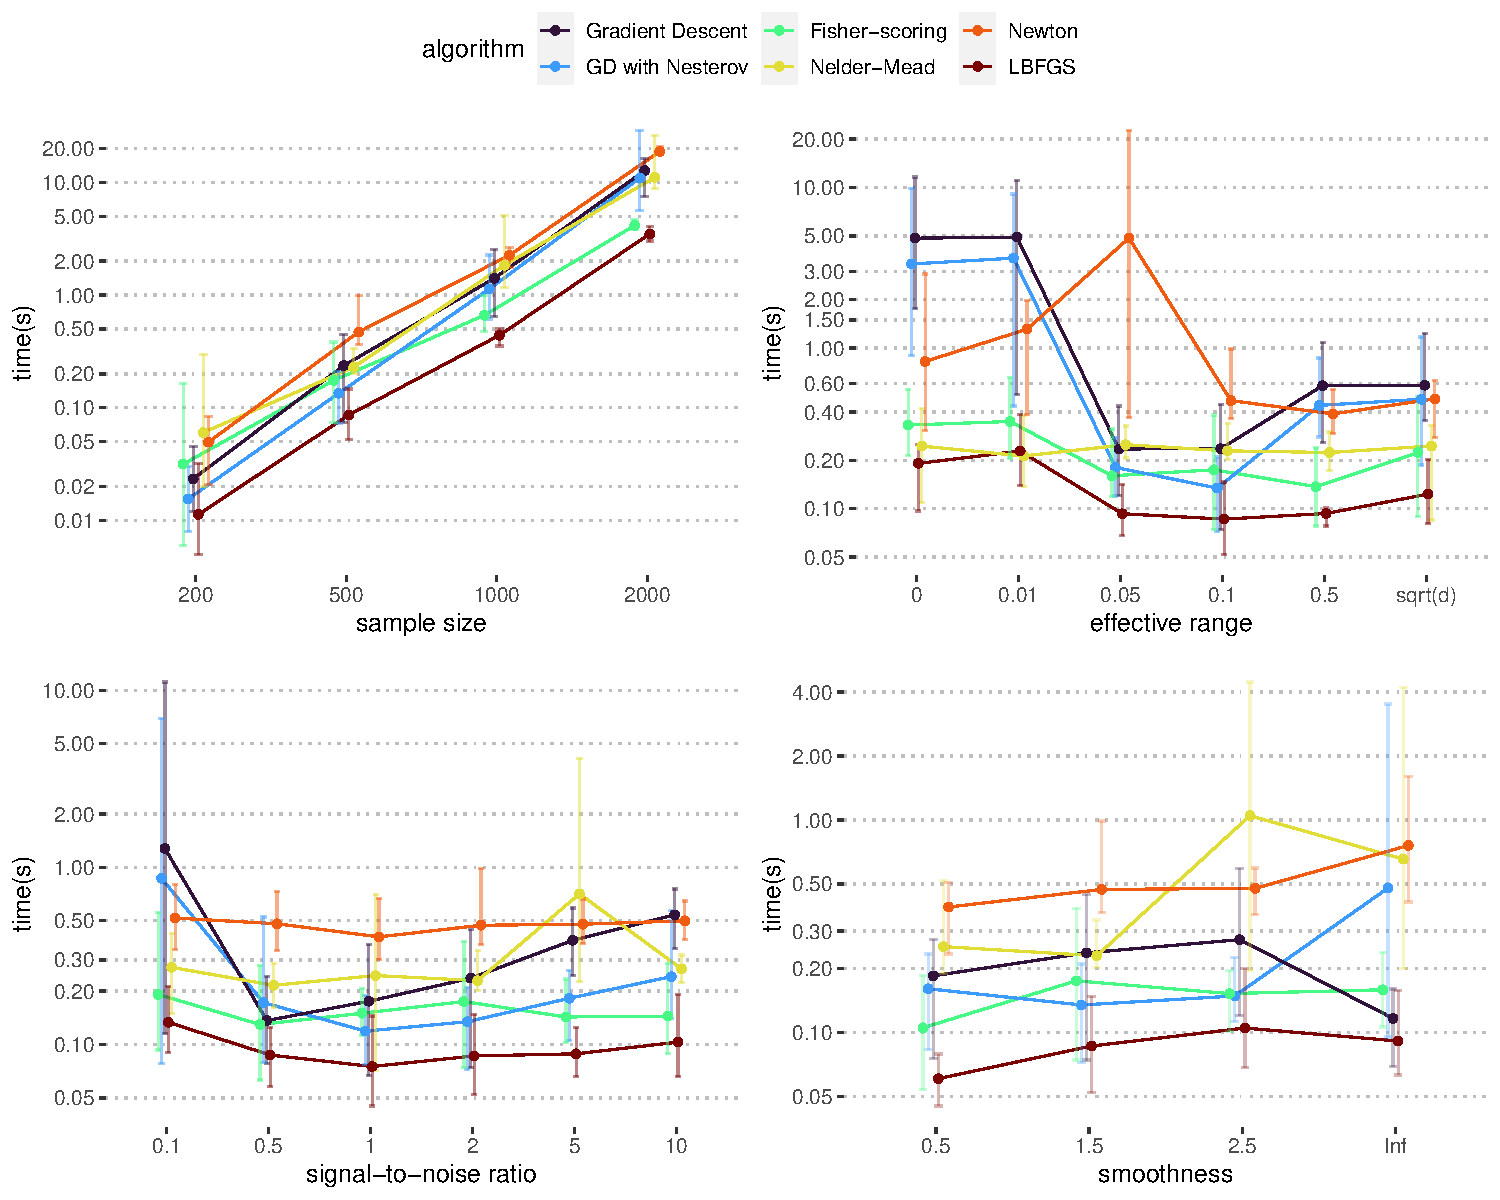
\includegraphics[width=.9\textwidth]{matern_0510} %<< no file extension
  %%         --- .5\textwidth stands for 50% of text width
  \caption[Times of simulated GP-Matern starting at default values: line graphs with range bars]%<<-- Legend for the list of figures at the beginning of you thesis
  {Comparison of optimization methods with different sample sizes and hyper-parameters $(n,\rho, \sigma^2_f/\sigma^2_n, \nu)$, all y-axes in $\log_{10}$ scale.}% legend displayed below the graph.
  \label{fig:matern_default}
\end{figure}

\begin{figure}[hbt!]%--- Picture 'H'ere, 'B'ottom or 'T'op; '!' 
  \centering
  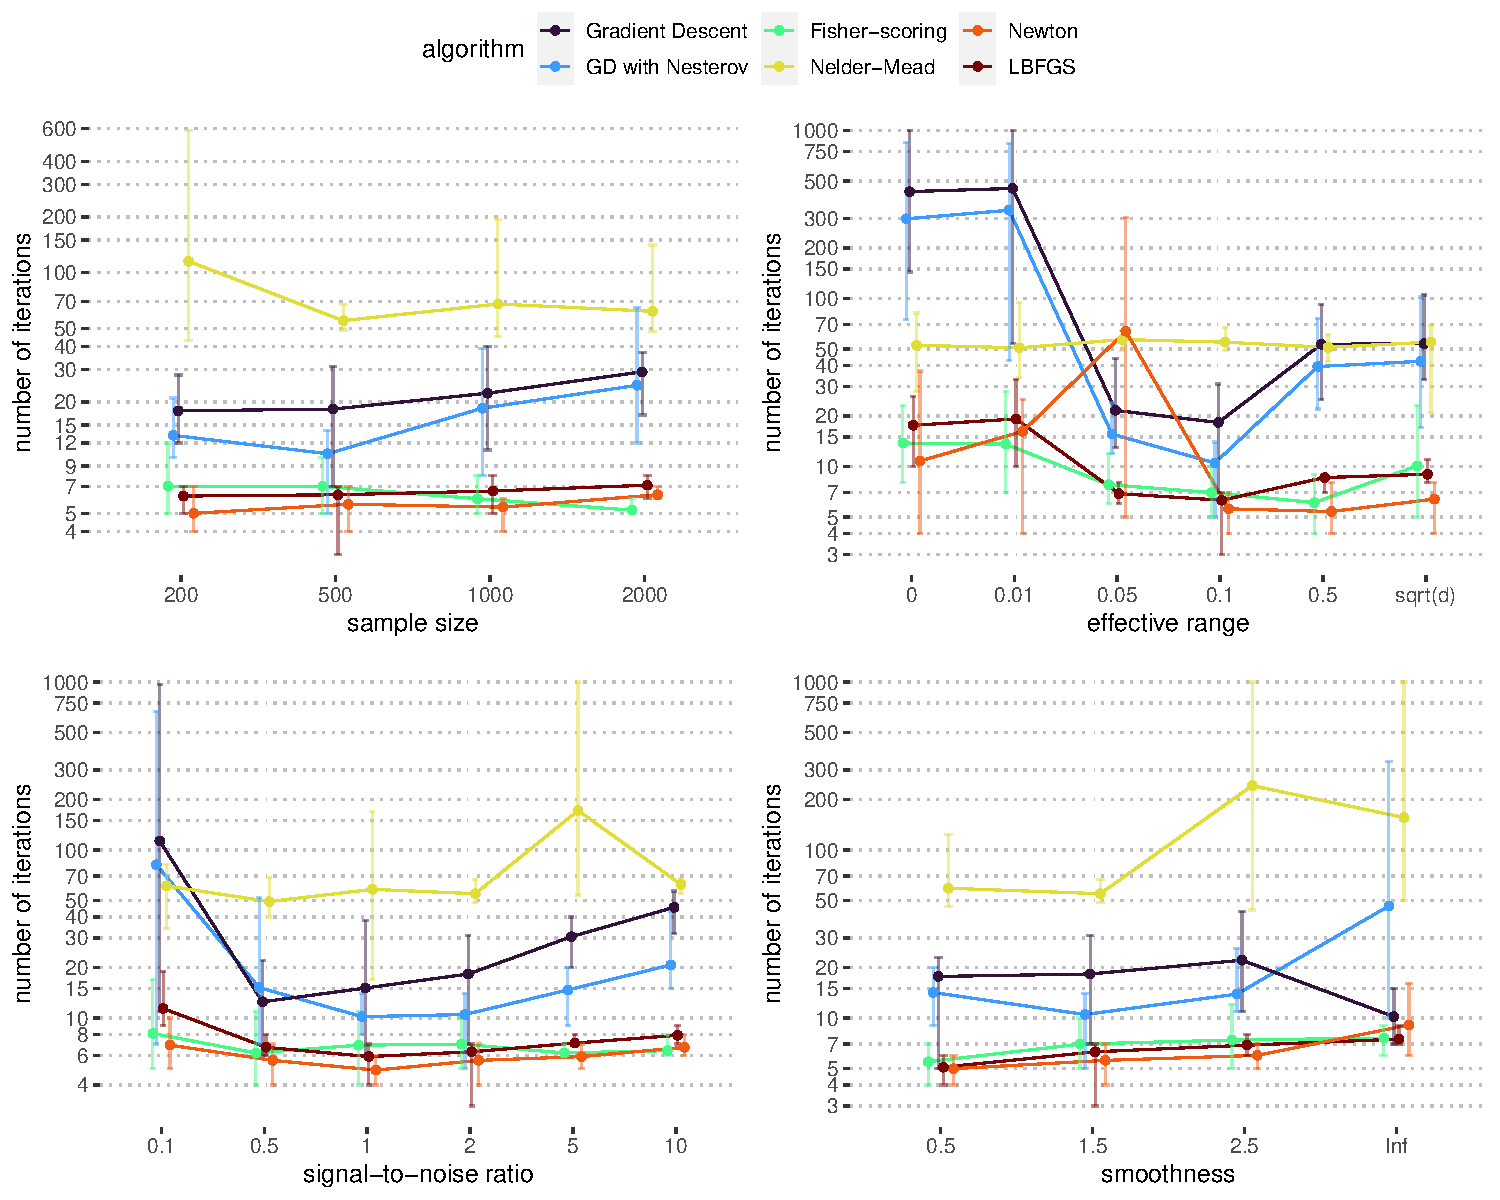
\includegraphics[width=.9\textwidth]{matern_iteration_0417} %<< no file extension
  %%         --- .5\textwidth stands for 50% of text width
  \caption[Number of iterations of simulated GP-matern starting at default values: line graphs with range bars]%<<-- Legend for the list of figures at the beginning of you thesis
  {Comparison of number of iterations of different methods, all y-axes are in $\log_{10}$ scale.}% legend displayed below the graph.
  \label{fig:matern_iteration}
\end{figure}

Figure 3.1 illustrates that LBFGS is the fastest method in most settings, and Fisher-scoring also has good performance. In most settings, Newton is the slowest method due to the need to compute the exact second derivative. 

Figure 3.2 shows that an iteration of Newton is more expensive, whereas an iteration of Nelder-Mead algorithm takes the least time. In each iteration, Newton calculates the exact second order derivative, and Nelder-Mead only evaluates the function values. Also, LBFGS, Newton, and Fisher-scoring methods mostly converge within 10 steps of iteration, and tend to require more steps in the case of small range parameter $\rho$. 

We check whether these optimization methods converge by checking the final log-likelihood values, and there are the following convergence problems:

\begin{itemize}
\item When $\rho=0$ (the simulated data is actually i.i.d Gaussian distributed), Nelder-Mead fails to converge in 2 (of 10) repetitions. 
\item When $\rho = 0.01$, Nelder-Mead fails in 3 (of 10) repetitions, Gradient Descent and GD with Nesterov accelerator both fail to converge in 2 (of 10) repetitions, Newton and LBFGS both fail in 1 (of 10) repetition.
\item When $\sigma^2_f/\sigma^2_n=0.1 \ (\sigma^2_n=10)$, Nelder-Mead fails to converge in 1 (of 10) repetition.
\item When $\sigma^2_f/\sigma^2_n=5 \ (\sigma^2_n=0.2)$, Nelder-Mead fails to converge in 1 (of 10) repetition.
\item When $\nu = 2.5$, Nelder-Mead fails to converge in 2 (of 10) repetitions.
\item When $\nu = \inf $, Nelder-Mead fails to converge in 1 (of 10) repetition.
\end{itemize}

We perform experiments with larger sample size with FITC and Vecchia approximations separately, resulting in four sets of experiment results in Figure 3.3. All repetitions of experiments result in successful convergence.

\begin{figure}[hbt!]%--- Picture 'H'ere, 'B'ottom or 'T'op; '!' 
  \centering
  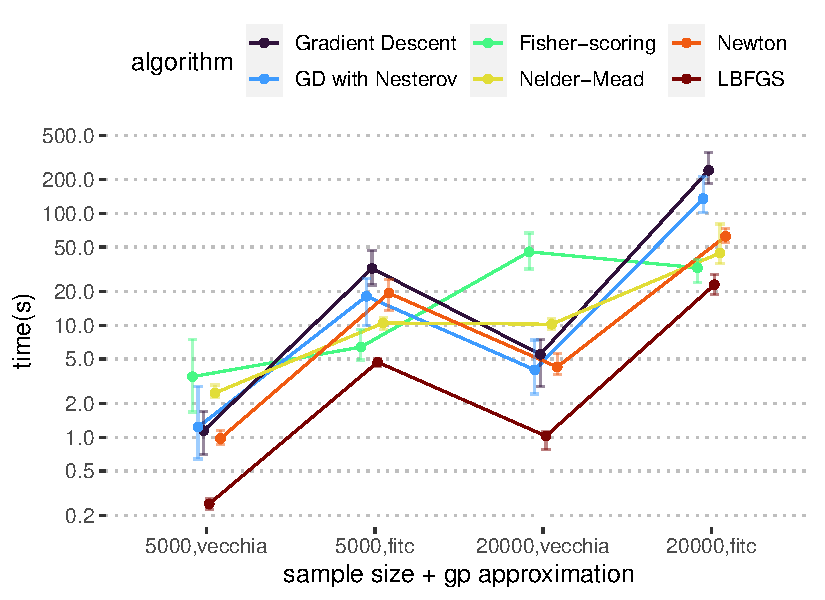
\includegraphics[width=.5\textwidth]{matern_approx_stable} %<< no file extension
  %%         --- .5\textwidth stands for 50% of text width
  \caption[Times of simulated GP-Matern using approximation: line graphs with range bars]%<<-- Legend for the list of figures at the beginning of you thesis
  {Comparison of times of different methods with approximation enabled, y-axis in $\log_{10}$ scale.}% legend displayed below the graph.
  \label{fig:matern_iteration}
\end{figure}

Figure 3.3 shows that LBFGS still outperforms the other methods with approximation enabled, and using the Vecchia approximation for GP models seems to be more efficient on average than FITC. LBFGS has the most stable performance, which can be deduced from the shorter vertical distances between bars. However, the approximate calculation of Fisher information with Vecchia in the implementation of \texttt{GPBoost} makes it slower than the other optimization methods, and in this sense, it is an unfair comparison between Fisher Scoring and other optimization methods in the presence of Vecchia approximation.

\subsubsection{Different initialization}
To investigate the influence of the starting points of the hyper-parameters on the optimization, we repeat the experiments in Figure 3.1, but with the starting values as true values and with inappropriately large values, which corresponds to the results in Figure 3.4 and Figure 3.5 respectively.

\begin{figure}[hbt!]%--- Picture 'H'ere, 'B'ottom or 'T'op; '!' Try to
                    %impose your will to LaTeX
  \centering
  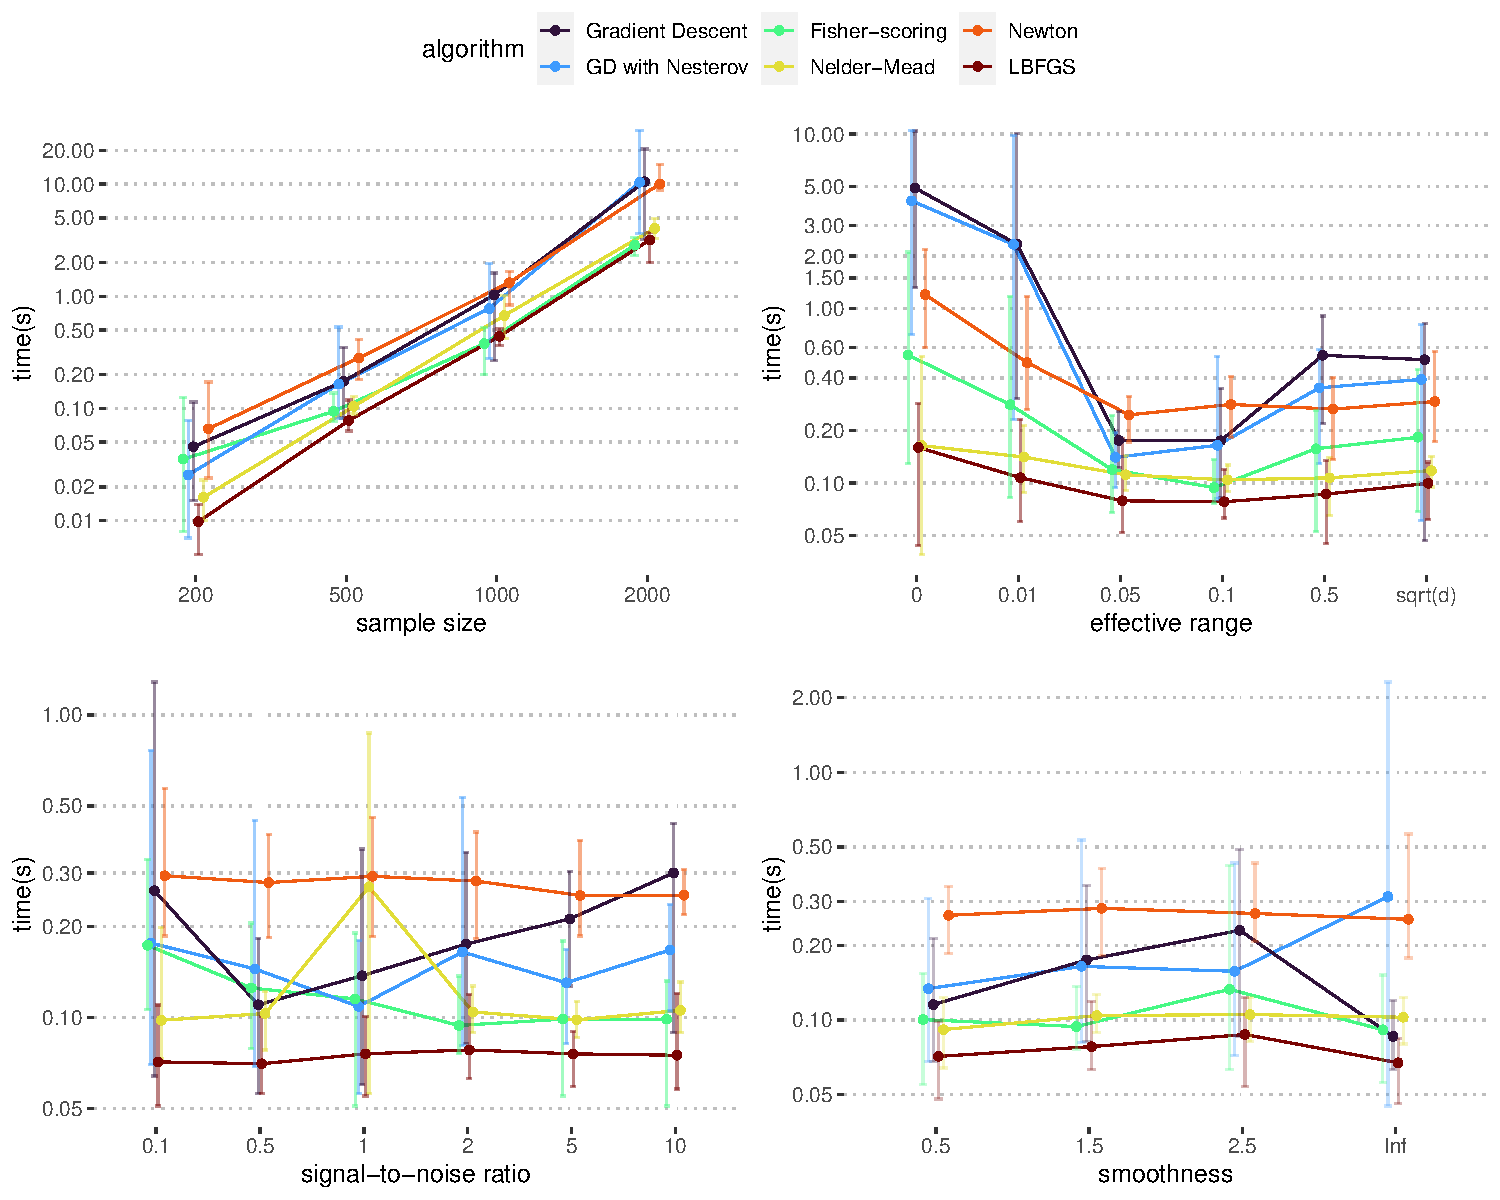
\includegraphics[width=.9\textwidth]{matern_init_true} %<< no file extension
  %%         --- .5\textwidth stands for 50% of text width
  \caption[Times of simulated GP-Matern starting at true values: line graphs with range bars]%<<-- Legend for the list of figures at the beginning of you thesis
  {Comparison of different optimization methods with different sample sizes and hyper-parameters, starting at true values, all y-axes in $\log_{10}$ scale.}
  \label{fig:matern_init_true}
\end{figure}

\begin{figure}[hbt!]%--- Picture 'H'ere, 'B'ottom or 'T'op; '!' Try to
                    %impose your will to LaTeX
  \centering
  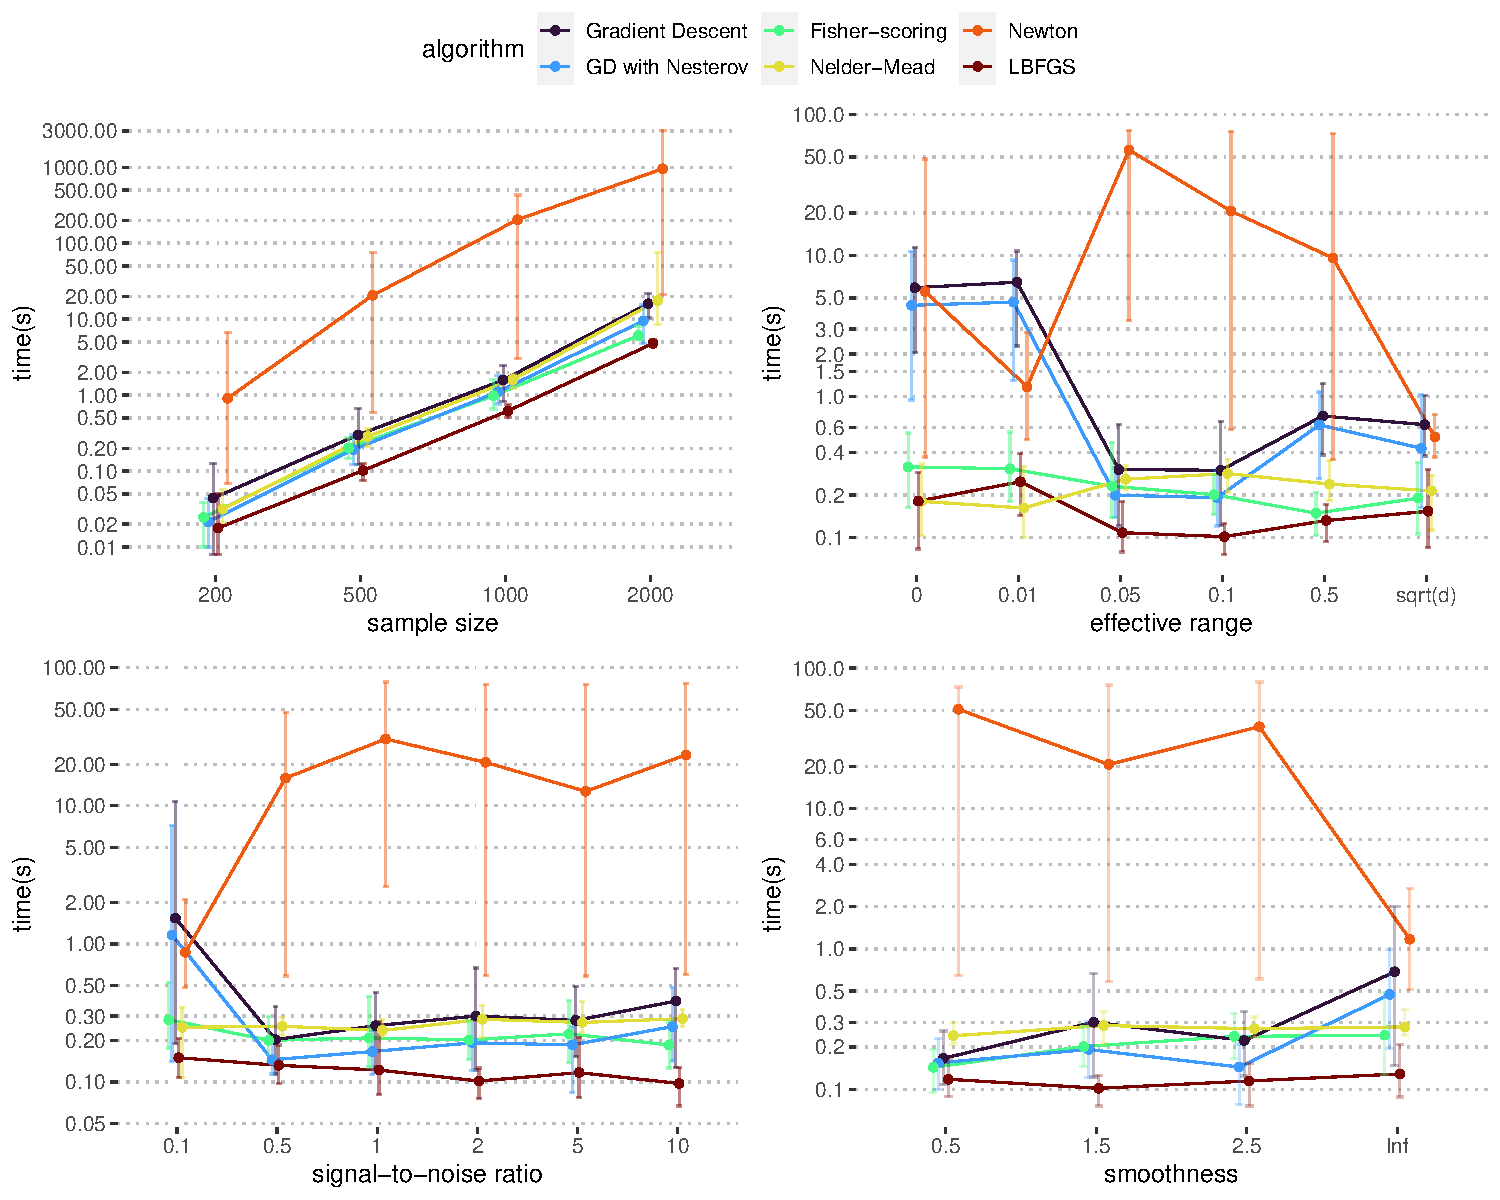
\includegraphics[width=.9\textwidth]{matern_init_unreas} %<< no file extension
  %%         --- .5\textwidth stands for 50% of text width
  \caption[Times of simulated GP-Matern starting at large values: line graphs with range bars]%<<-- Legend for the list of figures at the beginning of you thesis
  {Comparison of different algorithms with different sample sizes and hyper-parameters, starting at large values, 10 repetitions. All y-axes are in $\log 10$ scale.}% legend displayed below the graph.
  \label{fig:matern_init_unreas}
\end{figure}

Comparing Figures 3.4 and 3.5 with Figure 3.1, we can conclude that LBFGS is the fastest method in most experiments with any initialization strategy. Newton is sensitive to the choice of starting point, reflected by the phenomenon that starting from points far from the optima makes it difficult to converge within the iteration limit. However, if a suitable starting point is chosen, Fisher-scoring or Nelder-Mead can be as fast as LBFGS.

When starting the iteration from true values, all optimization methods successfully converge to the optima and consume less time compared to the other two initialization strategies. It is intuitive that the time of any optimizer will be longer if it starts iterating from an unreasonably distant point instead of a reasonable point related to the sample. Also, the convergence problem with unreasonable starting points in Figure 3.5 is more severe than with the default initialization:

\begin{itemize}
%\item Newton is manually excluded from experiments of $n=20000$ as it is extremely slow.
\item In the default setting ($n=500, \rho=0.1, \sigma^2_f/\sigma^2_n = 2$, and $\nu=1.5$), Newton fails to converge in 2 (of 10) repetitions.
\item When $n=1000$, Newton fails to converge in 4 (of 10) repetitions.
\item When $n=2000$, Newton fails to converge in 3 (of 10) repetitions.
%\item When $n=5000$, Newton fails in 8 (of 10) repetitions, Fisher-scoring fails to converge in 4 (of 10) repetitions.
\item When $\rho=0$, Nelder-Mead and LBFGS fails both in 1 (of 10) repetition.
\item When $\rho=0.01$, GD, GD with Nesterov accelerator and LBFGS all fails in 1 (of 10) repetition.
\item When $\rho=0.05$, Newton fails to converge in 7 (of 10) repetitions.
\item When $\rho=0.5$, Newton fails to converge in 1 (of 10) repetition.
\item When $\sigma^2_f/\sigma^2_n = 0.1$, Nelder-Mead and Newton both fail in 2 (of 10) repetitions.
\item When $\sigma^2_f/\sigma^2_n = 1$, Newton fails to converge in 2 (of 10) repetitions.
\item When $\sigma^2_f/\sigma^2_n = 5$, Newton fails to converge in 1 (of 10) repetition.
\item When $\sigma^2_f/\sigma^2_n = 5$, Newton fails to converge in 3 (of 10) repetitions.
\item When $\nu=0.5$, Newton fails in 5 (of 10) repetitions.
\item When $\nu=2.5$, Newton fails in 5 (of 10) repetitions.
\end{itemize}

\subsubsection{BFGS-based methods}

Considering the good performance of LBFGS, we further compare five variants of BFGS methods available in R. Two approximations are still enabled for large data. Besides ``lbfgs" in \texttt{GPBoost}, which we have experimented with, we also introduce ``lbfgs\_not\_profile \_out\_nugget" from \texttt{GPBoost}, and BFGS, L-BFGS-B and L-BFGS (L-BFGS-B with no bound on hyper-parameters) from \texttt{optim} function. 

The results are displayed in Figures 3.6 and 3.7, which show that ``lbfgs" is faster than ``lbfgs\_not\_profile\_out\_nugget", and they both significantly beat the three optimization methods in \texttt{optim}. In addition, some methods have convergence problems:

\begin{itemize}
    \item When $\rho=0$, L-BFGS-B(optim) fails to converge in 1 (of 10) repetition.
    \item When $\rho=0.01$, L-BFGS-B(optim) fails to converge in 3 (of 10) repetitions, ``lbfgs\_not\_profile\_out\_nugget" fails to converge in 2 (of 10) repetitions.
    \item When $\rho=\sqrt{2}$, BFGS(optim) fails to converge in 1 (of 10) repetition.
    \item When $\sigma^2_f/\sigma^2_n = 0.1$, L-BFGS-B(optim) fails to converge in 2 (of 10) repetitions.
    \item When $n=20000$ and using FITC approximation, BFGS(optim) fails to converge in 2 (of 10) repetitions.
\end{itemize}

\begin{figure}[hbt!]%--- Picture 'H'ere, 'B'ottom or 'T'op; '!' Try to
                    %impose your will to LaTeX
  \centering
  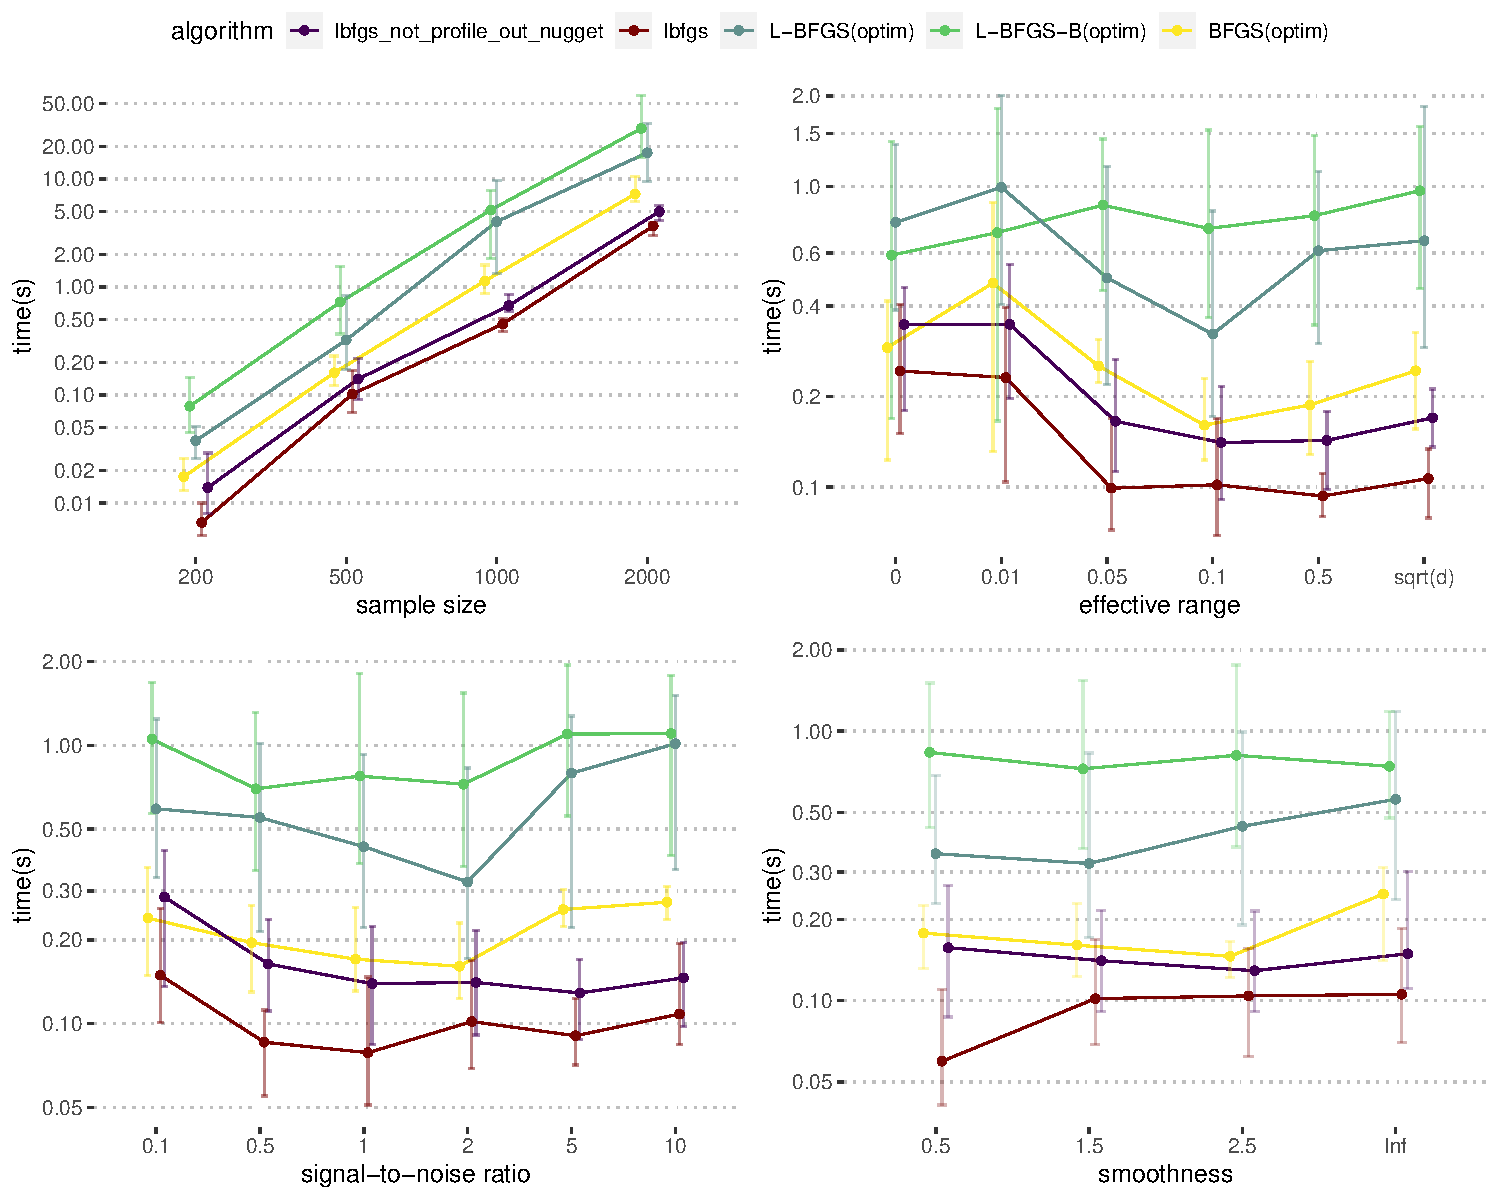
\includegraphics[width=.9\textwidth]{matern_bfgs_0606} %<< no file extension
  %%         --- .5\textwidth stands for 50% of text width
  \caption[Comparison of BFGS variants: times of GP-Matern starting at default values: line graphs with range bars]%<<-- Legend for the list of figures at the beginning of you thesis
  {Comparison of BFGS-based algorithms with different sample sizes and hyper-parameters, starting at default values, all Y-axes are in $\log_{10}$ scale.}% legend displayed below the graph.
  \label{fig:matern_bfgs}
\end{figure}

\begin{figure}[hbt!]%--- Picture 'H'ere, 'B'ottom or 'T'op; '!' 
  \centering
  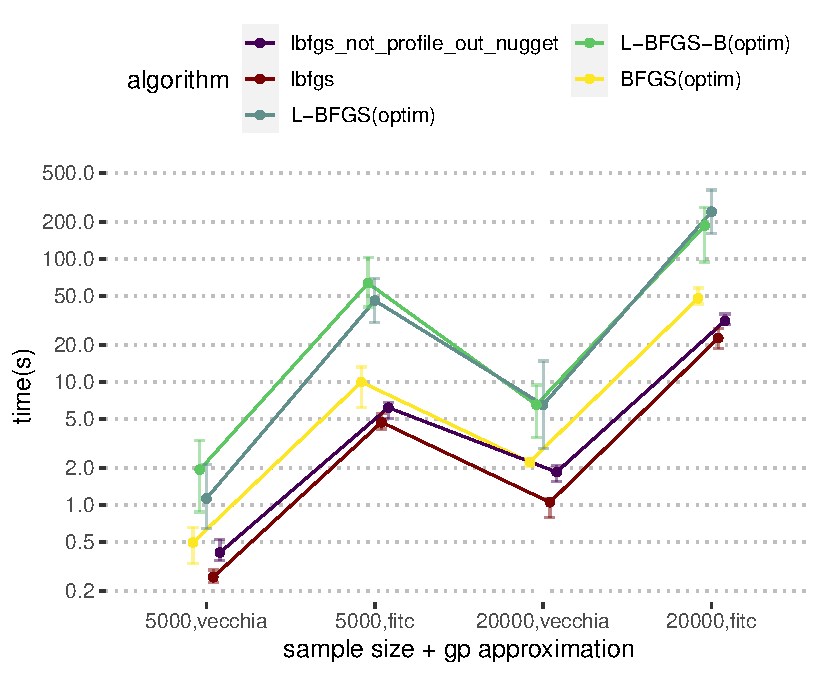
\includegraphics[width=.5\textwidth]{bfgs_approx_stable} %<< no file extension
  %%         --- .5\textwidth stands for 50% of text width
  \caption[Comparison of BFGS variants with approximation: times of GP-Matern starting at default values: line graphs with range bars]%<<-- Legend for the list of figures at the beginning of you thesis
  {Comparison of times of BFGS methods with approximation on zero-mean GP models, y-axis in $\log_{10}$ scale.}% legend displayed below the graph.
  \label{fig:linear_iteration}
\end{figure}


\subsection{GP with Non-zero mean}

To further investigate the performance of the optimization methods on GP models, we add the linear regression term $\boldsymbol{Z\beta}$ as the mean function $m(\bold{x})$:

\begin{equation}
    \pmb{z} = [1, z_{1},...,z_{9}], \ \boldsymbol{\beta} = [0,1,...,1] \text{, where } z_{i}\overset{\mathrm{iid}}{\sim} N(0, 0.1).
\end{equation}

Now we need to estimate the hyper-parameters $(\rho, \sigma^2_f, \sigma^2_n)$ and the linear coefficients $\boldsymbol{\beta}$. The experimental settings of hyper-parameters in section 3.1.1 are applied again. The experimental results are shown in Figure 3.8, and the large scale optimization results are shown in Figure 3.9. Note that Nelder-Mead method is excluded because it is unable to converge to the optima in any setting, and it takes a long time to search in each step. The heuristic search strategy of Nelder-Mead makes it difficult to solve the problem when the number of parameters to be estimated increases enormously. 

\begin{figure}[hbt!]%--- Picture 'H'ere, 'B'ottom or 'T'op; '!' Try to
                    %impose your will to LaTeX
  \centering
  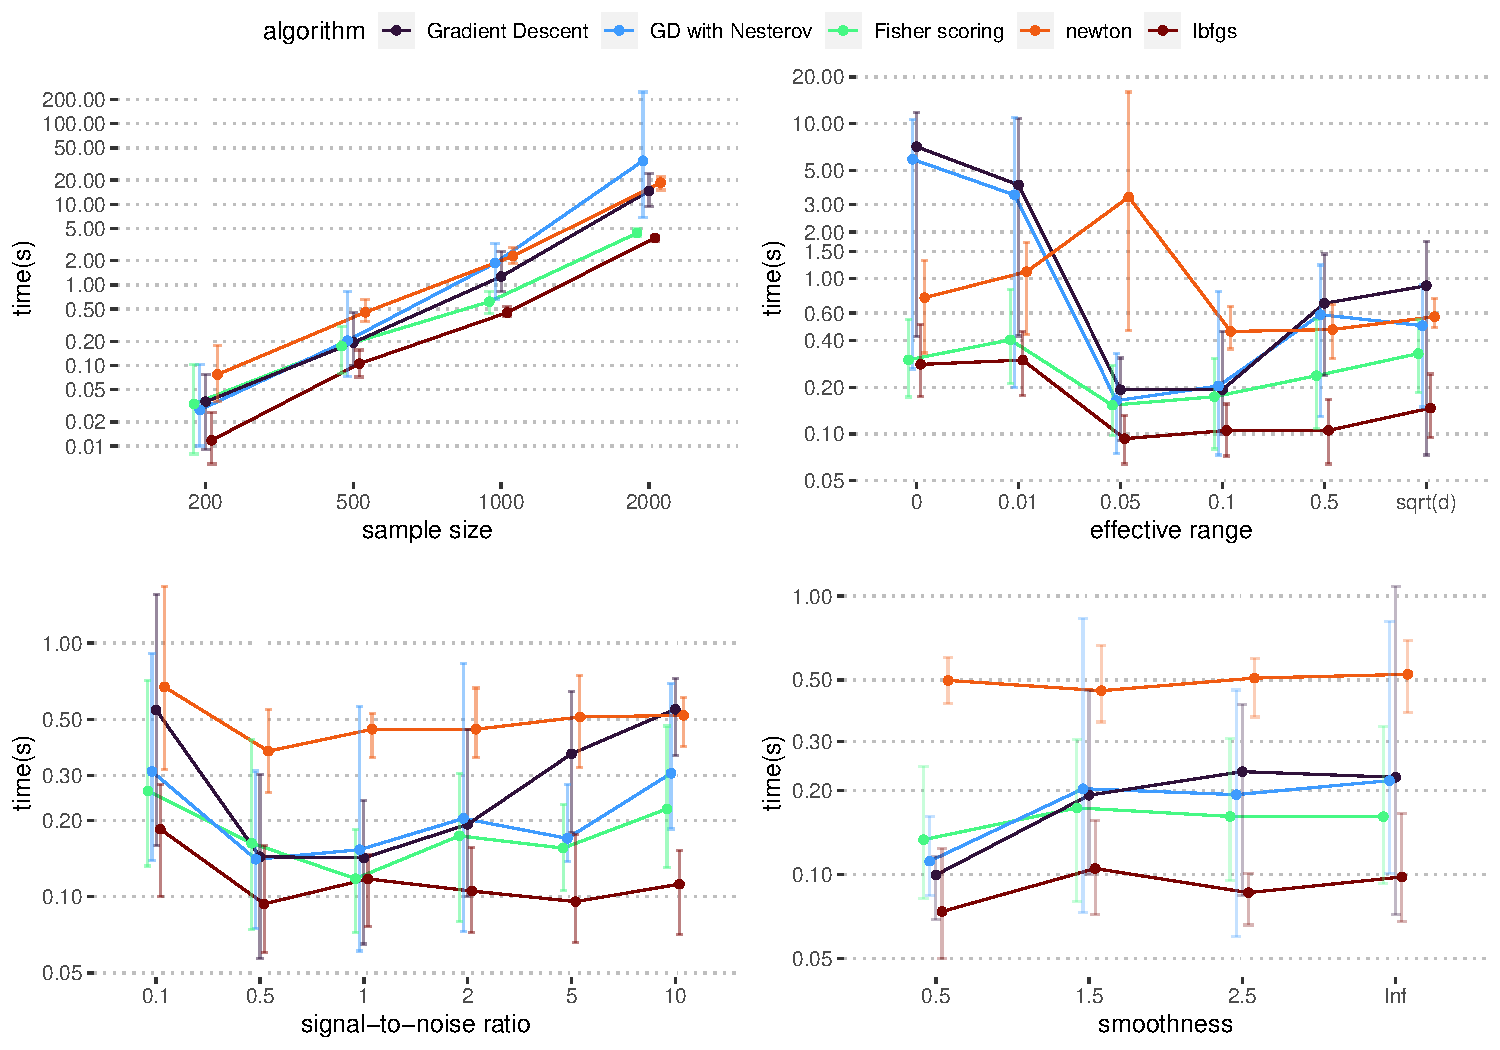
\includegraphics[width=.9\textwidth]{matern_linear_reg} %<< no file extension
  %%         --- .5\textwidth stands for 50% of text width
  \caption[Times of GP-Matern with linear regression terms: line graphs with range bars]%<<-- Legend for the list of figures at the beginning of you thesis
  {Comparison of different methods of GP models with added linear regression term, default starting values, all y-axes are in $\log_{10}$ scale.}
  \label{fig:matern_linear}
\end{figure}

Compared to the results of the zero-mean GP models in Figure 3.1, Figure 3.8 shows that the relative ranking among the optimization methods and the average time used by each method remain the same after introducing the linear regression term, and LBFGS still has outstanding performance. Results in Figure 3.9 show that LBFGS and Newton take the least time in large scale optimization.

The convergence check shows that:
\begin{itemize}
    \item When $\rho=0.01$, GD, GD with Nesterov accelerator and Newton all fail to converge in 1 (of 10) repetition.
    \item When $n=5000$ and using Vecchia approximation, Newton's method fails to converge in 1 (of 10) repetition.
\end{itemize}

\begin{figure}[hbt!]%--- Picture 'H'ere, 'B'ottom or 'T'op; '!' 
  \centering
  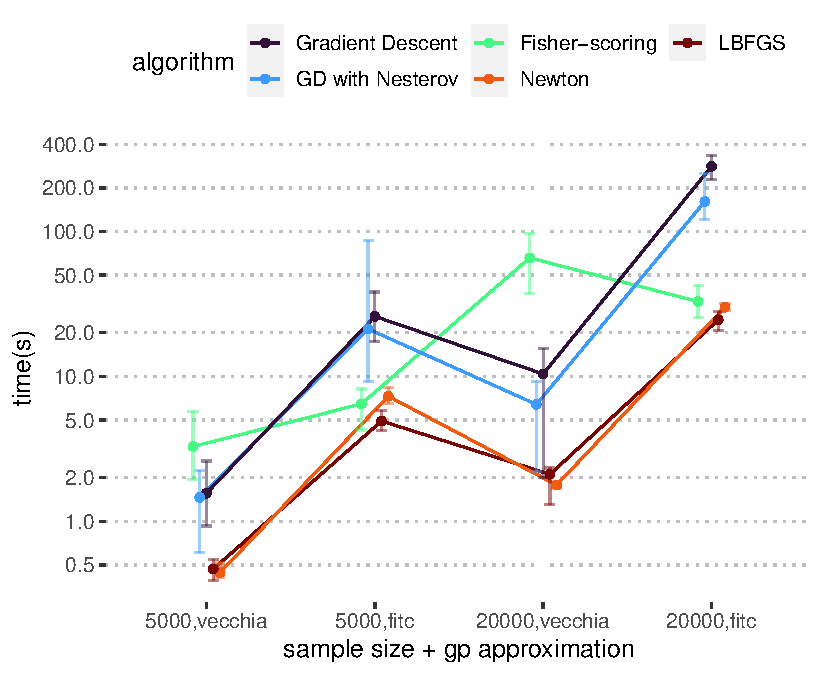
\includegraphics[width=.5\textwidth]{linear_approx_stable} %<< no file extension
  %%         --- .5\textwidth stands for 50% of text width
  \caption[Times of GP-Matern with linear regression term using approximation: line graphs with range bars]%<<-- Legend for the list of figures at the beginning of you thesis
  {Comparison of times of different methods with approximation on model with linear terms, y-axis in $\log_{10}$ scale.}% legend displayed below the graph.
  \label{fig:linear_iteration}
\end{figure}

\subsection{Binary data}

The observation variables are categorical in some applications, where GP classification models are applied. Therefore, we test the performance of optimization methods on GP models with binary likelihood (Bernoulli distribution with \textit{logit} link function). In this section, similar settings of hyper-parameters are used, whereas the noise term is no longer included in the data simulation. Instead of the signal-to-noise ratio, we only change the signal variance in the experiment. The results are displayed in Figurea 3.10 and 3.11, note that Fisher-scoring is excluded in the results, because the Fisher information is not computable for GP with binary likelihood. The convergence check shows that, when $n=5000$ and using FITC approximation, Newton fails to converge in 1 (of 10) repetition.

\begin{figure}[hbt!]%--- Picture 'H'ere, 'B'ottom or 'T'op; '!' Try to
                    %impose your will to LaTeX
  \centering
  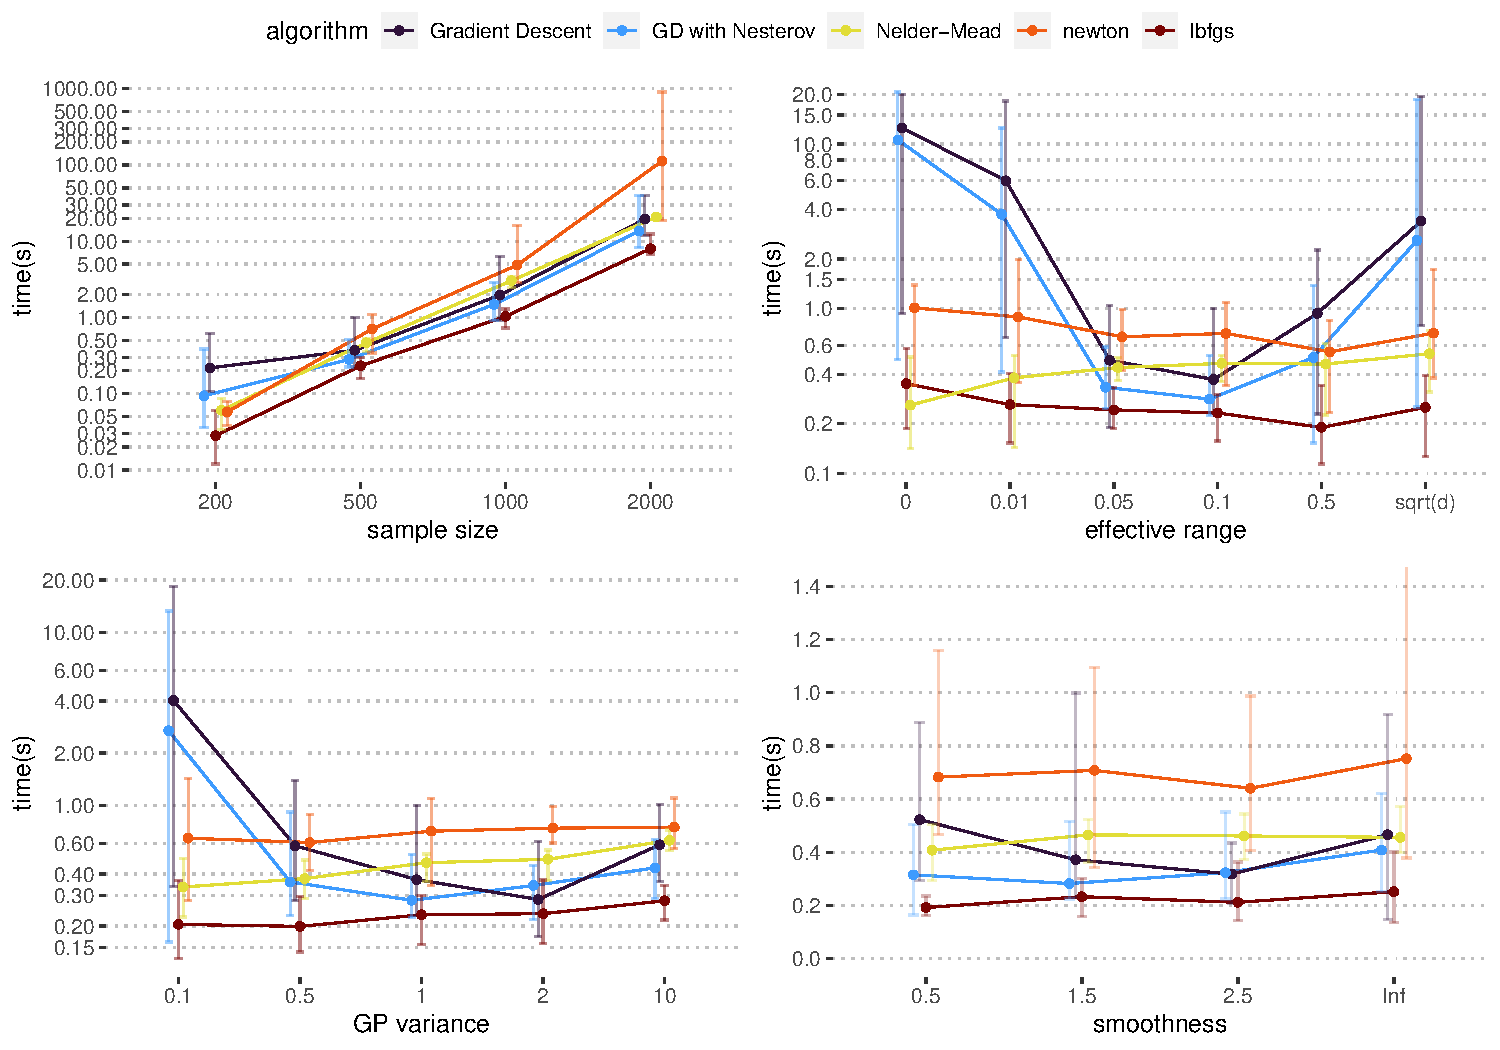
\includegraphics[width=.9\textwidth]{matern_binary_0426} %<< no file extension
  %%         --- .5\textwidth stands for 50% of text width
  \caption[Times of GP-Matern with Binary likelihood: line graphs with range bars]%<<-- Legend for the list of figures at the beginning of you thesis
  {Comparison of methods on GP with binary likelihood of different sample sizes and hyper-parameters, all y-axes except lower-right sub-figure are in $\log_{10}$ scale.}% legend displayed below the graph.
  \label{fig:matern_binary}
\end{figure}

\begin{figure}[hbt!]%--- Picture 'H'ere, 'B'ottom or 'T'op; '!' 
  \centering
  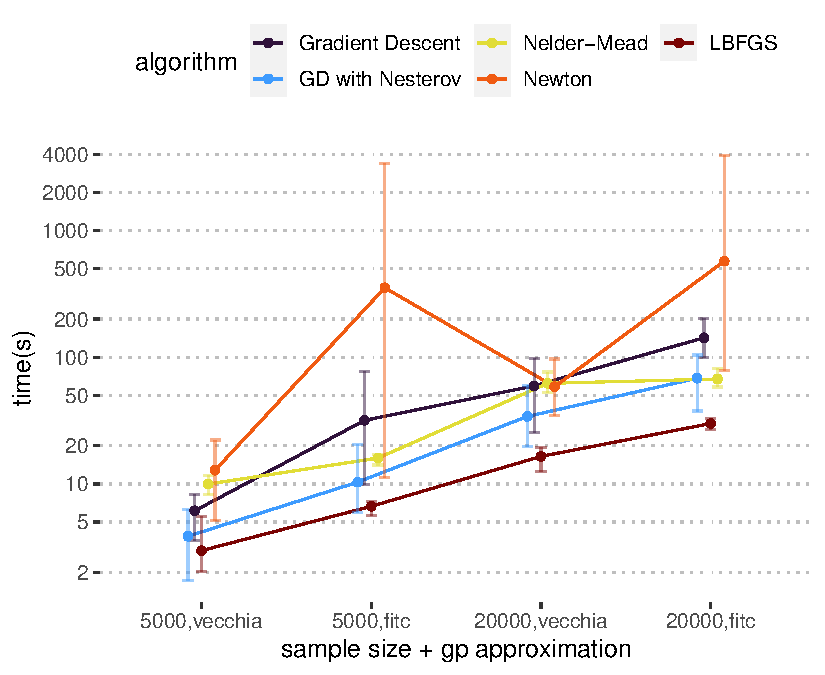
\includegraphics[width=.5\textwidth]{binary_approx_stable} %<< no file extension
  %%         --- .5\textwidth stands for 50% of text width
  \caption[Times of  GP-Matern with binary likelihood using approximation: line graphs with range bars]%<<-- Legend for the list of figures at the beginning of you thesis
  {Comparison of times of different methods with approximation on model with binary likelihood, y-axis in $\log_{10}$ scale.}% legend displayed below the graph.
  \label{fig:linear_iteration}
\end{figure}

Furthermore, we again add the linear regression terms as in Eq.(5) into the GP classification models. The performance comparison of four algorithms (GD, GD with Nesterov accelerator, Nelder Mead, and LBFGS) is displayed in Figure 3.12 and Figure 3.13. In these experiments, Newton's method faces some convergence problems:

\begin{itemize}
    \item When $\rho=0.01$, Newton fails to converge in 1 (of 10) repetition.
    \item When $\sqrt d$, Newton fails to converge in 1 (of 10) repetition.
    \item When n=20000 and using FITC approximation, Newton fails to converge in 2 (of 10) repetitions.
\end{itemize}

\begin{figure}[hbt!]%--- Picture 'H'ere, 'B'ottom or 'T'op; '!' Try to
                    %impose your will to LaTeX
  \centering
  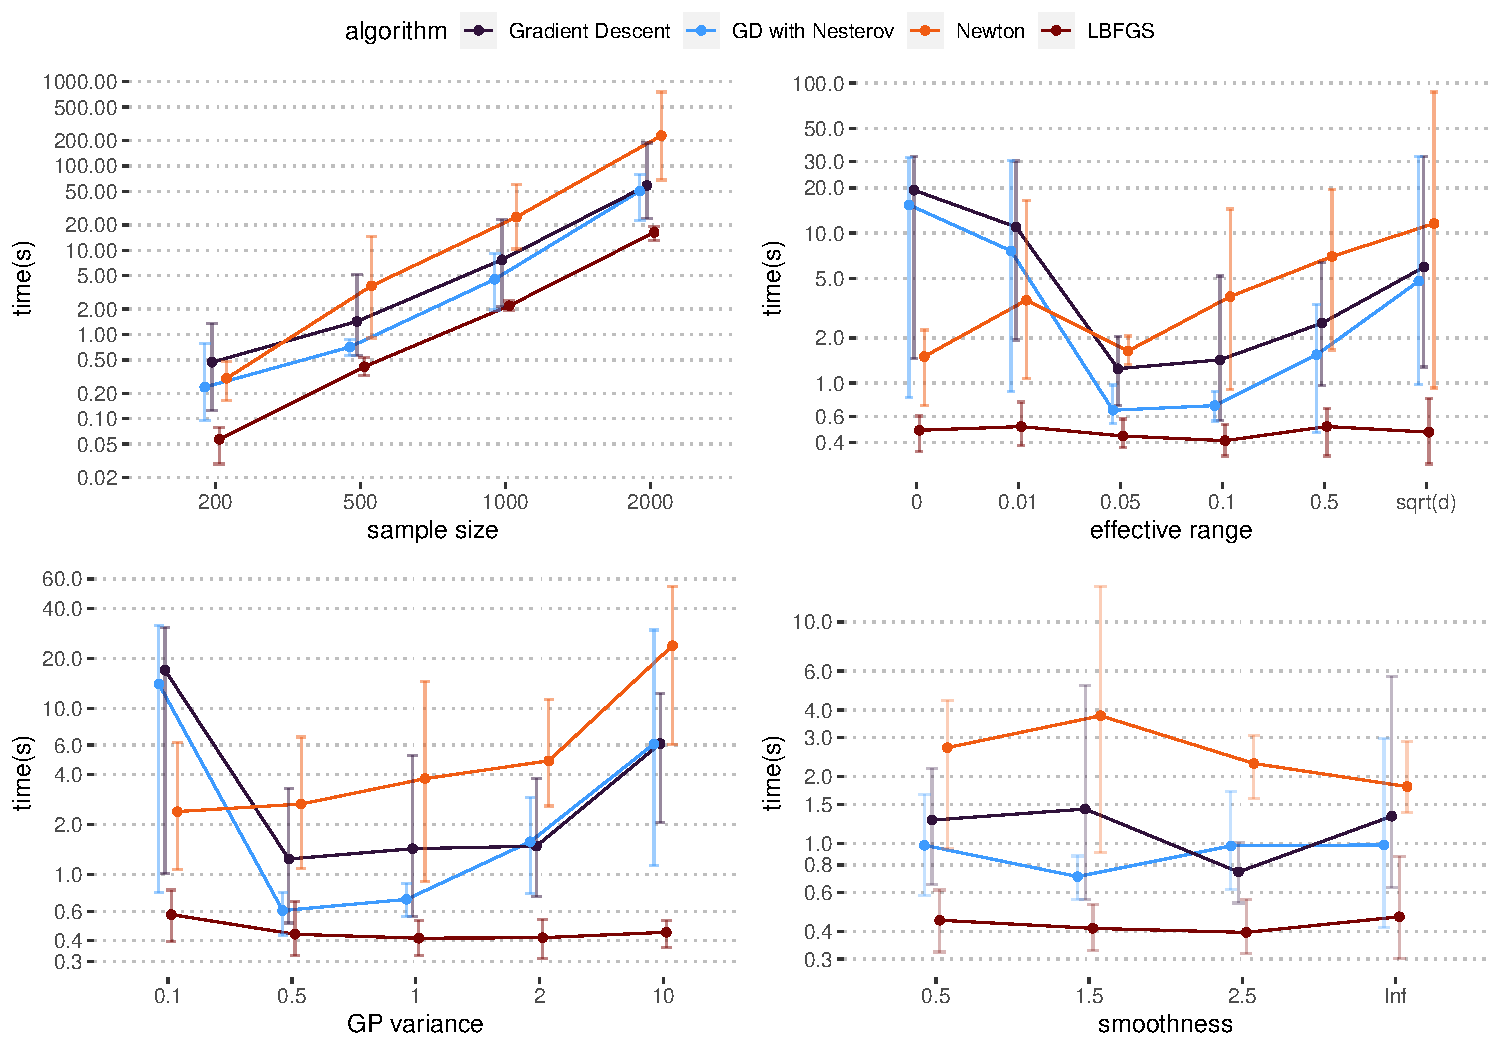
\includegraphics[width=.9\textwidth]{binary_linear_0426} %<< no file extension
  %%         --- .5\textwidth stands for 50% of text width
  \caption[Times of GP-Matern with Binary likelihood and linear regression terms: line graphs with range bars]%<<-- Legend for the list of figures at the beginning of you thesis
  {Comparison of different methods on GP with binary likelihood and added linear regression terms, all y-axes are in $\log_{10}$ scale.}% legend displayed below the graph.
  \label{fig:binary_linear}
\end{figure}

\begin{figure}[hbt!]%--- Picture 'H'ere, 'B'ottom or 'T'op; '!' 
  \centering
  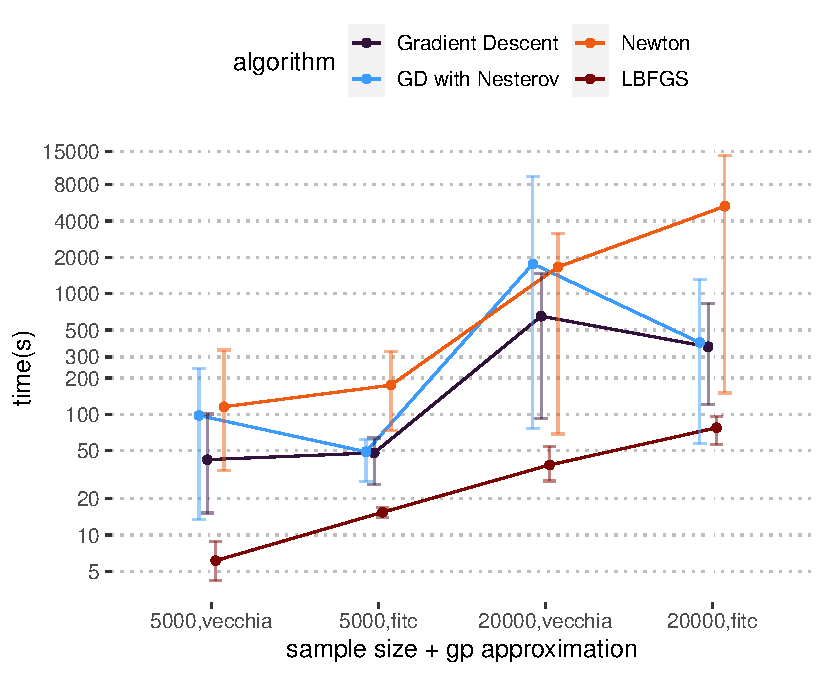
\includegraphics[width=.5\textwidth]{binary_linear_approx_stable} %<< no file extension
  %%         --- .5\textwidth stands for 50% of text width
  \caption[Times of GP-Matern with binary likelihood and linear regression terms using approximation: line graphs with range bars]%<<-- Legend for the list of figures at the beginning of you thesis
  {Comparison of times of different methods with approximation on model with binary likelihood and linear regression terms, y-axis in $\log_{10}$ scale.}% legend displayed below the graph.
  \label{fig:linear_iteration}
\end{figure}

From Figures 3.10, 3.11, 3.12 and 3.13 in this section, similar conclusions can be drawn; LBFGS is still excellent, followed by Nelder-Mead method and two GD methods, and Newton's method is the slowest one in most cases and shows instability, which is reflected by the large gap between maximum and minimum times. Gradient Descent methods are limited by the long-ridge and flat likelihood, which is illustrated by the slower optimization in the models with small range.

\section{Mis-specified models}

In Section 3.1, we have performed several experiments based on the GP models with Mat\'ern class covariance function, when we have used correctly specified models in the model fitting stage. In this section, performance of optimization methods in the situation of model mis-specification will be compared, which means that the GP model used for fitting belongs to a different distribution class than the model used for data simulation. In our experiments, the data sample is simulated from GP with Mat'ern covariance function with smoothness $\nu = 0.5/ \inf$, and then optimized using the GP model with different smoothness value.

Again, we consider the application of a smaller sample and a large sample of size 5000 (using Vecchia and FITC) and fit a GP model with different smoothness values. The results of data simulated by GP models with smoothness $\nu=0.5$ (exponential covariance) are shown in Figure 3.14. Figure 3.15 displays the results of smoothness $\nu \xrightarrow{} \infty$ (squared exponential or Gaussian covariance). The figures are divided into two parts: left for the experiments with smaller sample size, right for the large sample with Vecchia and FITC approximation.

\begin{figure}[hbt!]%--- Picture 'H'ere, 'B'ottom or 'T'op; '!' Try to
                    %impose your will to LaTeX
  \centering
  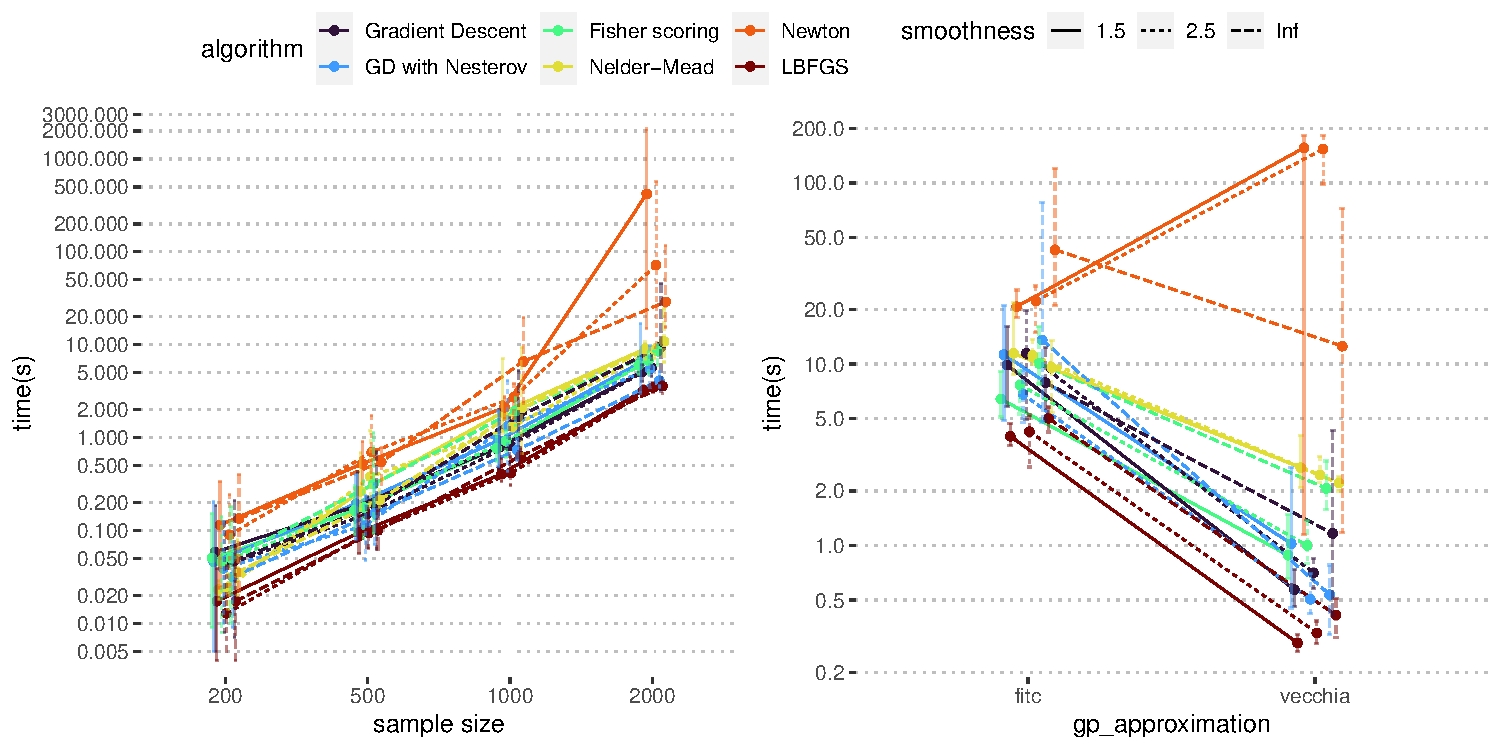
\includegraphics[width=.9\textwidth]{misspec_0.5_stable} %<< no file extension
  %%         --- .5\textwidth stands for 50% of text width
  \caption[Times of mis-specified GP with 0.5 smoothness: graphs of different line types with range bars]%<<-- Legend for the list of figures at the beginning of you thesis
  {Comparison of different methods using mis-specified GP models on data from GP with 0.5 smoothness, default starting values, 10 repetitions. Y-axis is in $\log 10$ scale. Vecchia approximation is utilized when n = 5000}% legend displayed below the graph.
  \label{fig:matern_mis_0.5}
\end{figure}

Figure 3.14 shows that LBFGS has the best performance with any smoothness parameters, and Newton is the slowest. The convergence check of this figure shows that for large data of 5000 points:

\begin{itemize}
    \item When $\nu=1.5$ and using Vecchia approximation, Newton fails to converge in 7 (of 10) repetitions.
    \item When $\nu=2.5$ and using Vecchia approximation, Newton fails to converge in 5 (of 10) repetitions.
\end{itemize} 

\begin{figure}[hbt!]%--- Picture 'H'ere, 'B'ottom or 'T'op; '!' Try to
                    %impose your will to LaTeX
  \centering
  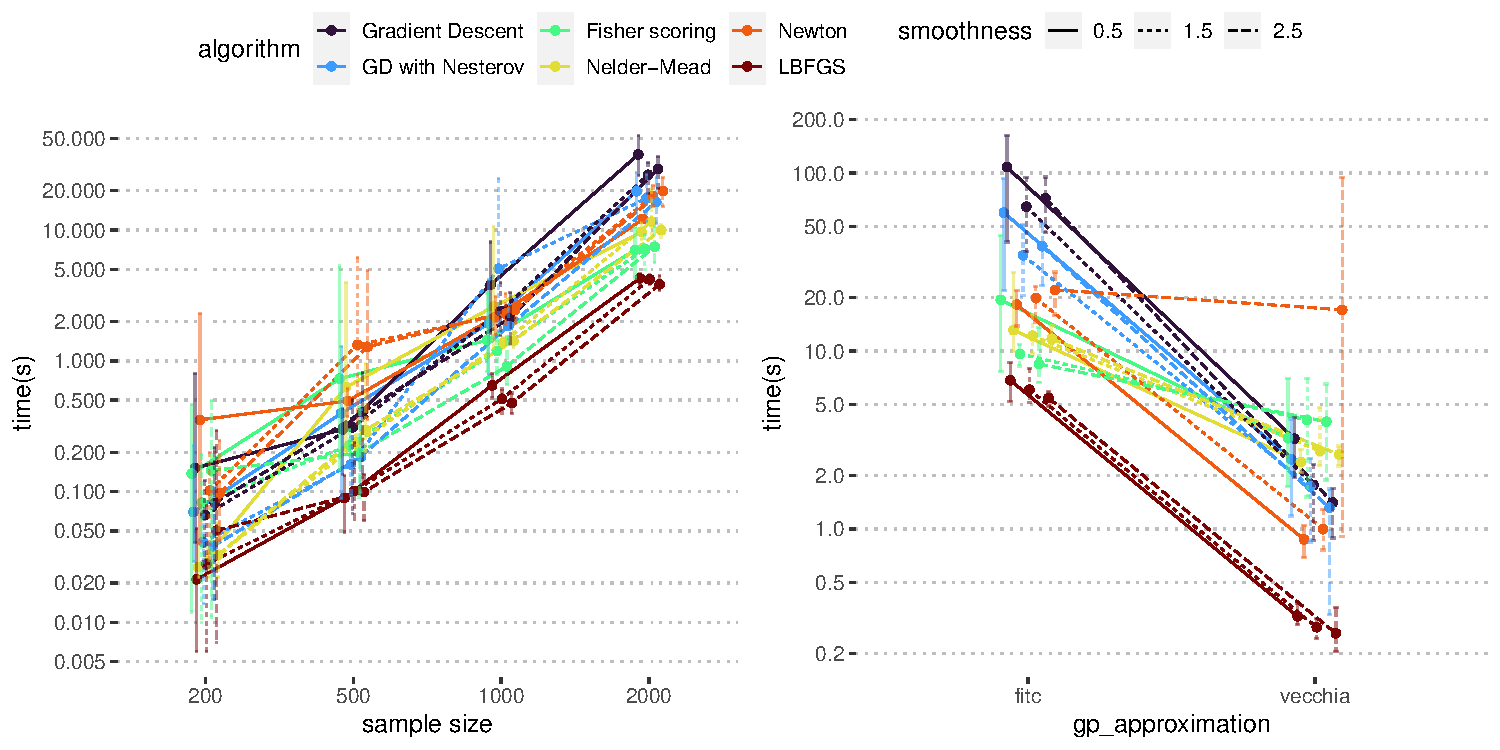
\includegraphics[width=.9\textwidth]{misspec_inf_stable} %<< no file extension
  %%         --- .5\textwidth stands for 50% of text width
  \caption[Times of mis-specified GP with infinite smoothness: graphs of different line types with range bars]
  {Comparison of different methods using mis-specified GP models on data from GP with infinite smoothness, default starting values, 10 repetitions. Y-axis is in $\log 10$ scale. Vecchia approximation is utilized when n = 5000.}
  \label{fig:matern_mis_Inf}
\end{figure}

bFor experiments of data from GP model of Gaussian covariance (infinite smoothness value), the convergence check shows that:

\begin{itemize}
    \item When $\nu=0.5, n=200$, Newton fails to converge in 6 (of 10) repetitions.
    \item When $\nu=0.5, n=500$, Nelder-Mead fails to converge in 1 (of 10) repetition.
\end{itemize} 
 
\section{Deterministic functions}

In this section, we introduce three deterministic functions for simulation experiments: Branin, Borehole and Piston (\cite{simulationlib}), and compare the performance of the optimization methods. We sample data from the functions and estimate the hyper-parameters of the Mat\'ern covariance function. This is the case when not enough information is known about the underlying function and the fitting model does not belong to the same distribution family as the true model. Note that in all deterministic experiments, the data is centered first in the pre-processing. We will first experiment with data of size 1000, and in section 3.3.4 we will use the Vecchia approximation for experiments on large data of size 20000.

\subsection{Branin function}
Branin function is a 2-dimensional function that usually evaluated over the domain $[-5,10]\times[0,15]$. It is defined as:

\begin{equation}
    f(\pmb{x}) = a(x_2 - bx_1^2 + cx_1 - r)^2 + s(1 - t) \cos{x_1} + s
\end{equation}
and we take the recommended value as $a = 1, b = 5.1/4\pi^2, c = 5/\pi, r = 6, s = 10$, and $t = 1/8\pi$ from \cite{simulationlib}.

Experiment results in Figure 3.16 illustrate that, even with Nesterov accelerator, Gradient Descent algorithm needs significantly more time to converge, especially when smoothness is 1.5 or 2.5. LBFGS remains the fastest in all cases. The convergence check of Branin experiment shows that, when $\nu\xrightarrow{} \infty$, Newton's method fails to converge in 3 (of 10) repetitions.

\begin{figure}[hbt!]%--- Picture 'H'ere, 'B'ottom or 'T'op; '!' Try to
                    %impose your will to LaTeX
  \centering
  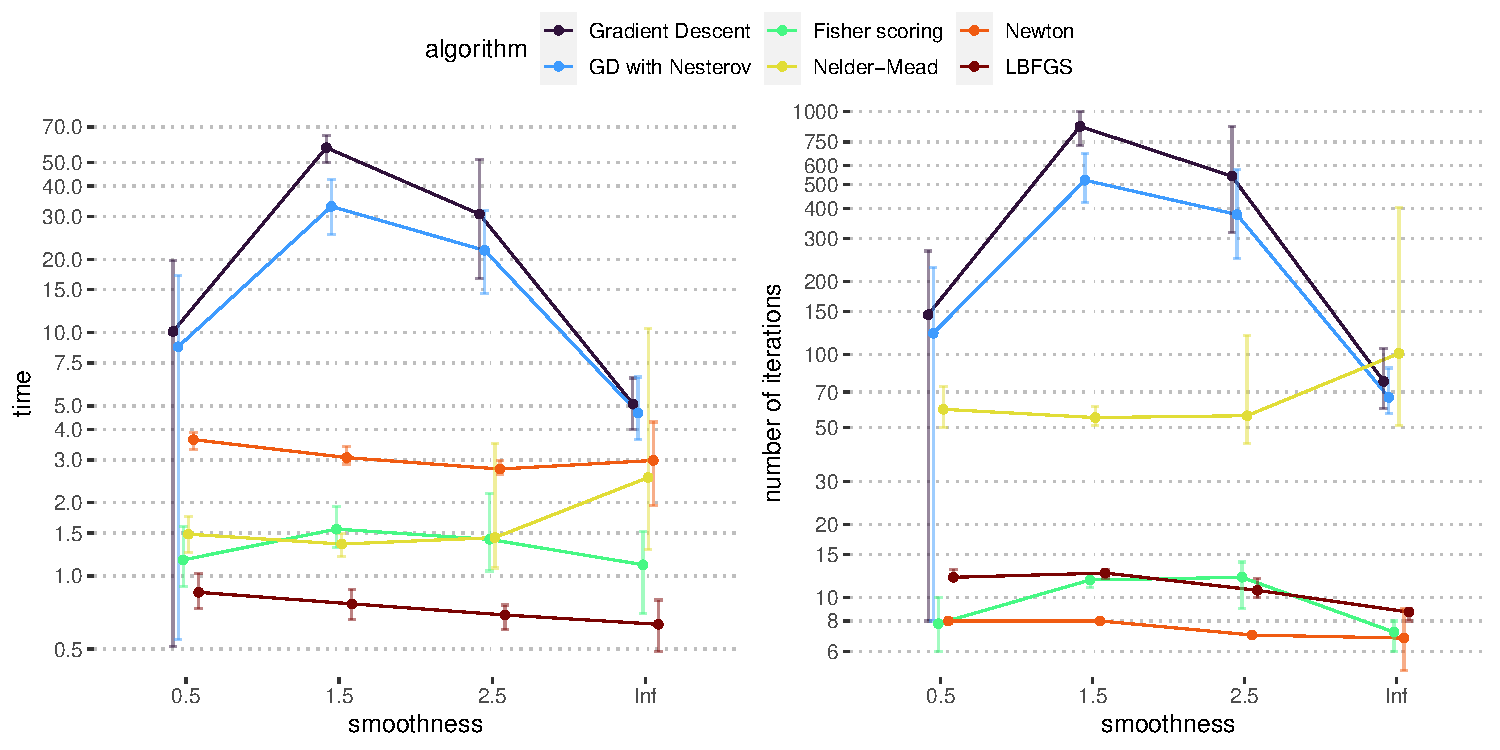
\includegraphics[width=.9\textwidth]{Branin_comparison_0426} %<< no file extension
  %%         --- .5\textwidth stands for 50% of text width
  \caption[Times of Branin function: line graphs with range bars]%<<-- Legend for the list of figures at the beginning of you thesis
  {Comparison of different methods using mis-specified GP models on data from Branin function, default starting values, 10 repetitions. Y-axes are in $\log 10$ scale.}% legend displayed below the graph.
  \label{fig:plotset}
\end{figure}

\subsection{Borehole function}
Borehole function models the flow of water through a borehole and it consists of eight input variables. Similar conclusions could be drawn from the results in Figure 3.17, except that Newton's method takes the longest average time with a large range when smoothness is 0.5. 

The convergence check shows that, when $\nu=0.5$, Newton algorithm fails to converge in 2 (of 10) repetitions. In these cases, Newton's method fails to find the optima within the prescribed of 1000 iterations limit.

\begin{figure}[hbt!]%--- Picture 'H'ere, 'B'ottom or 'T'op; '!' 
  \centering
  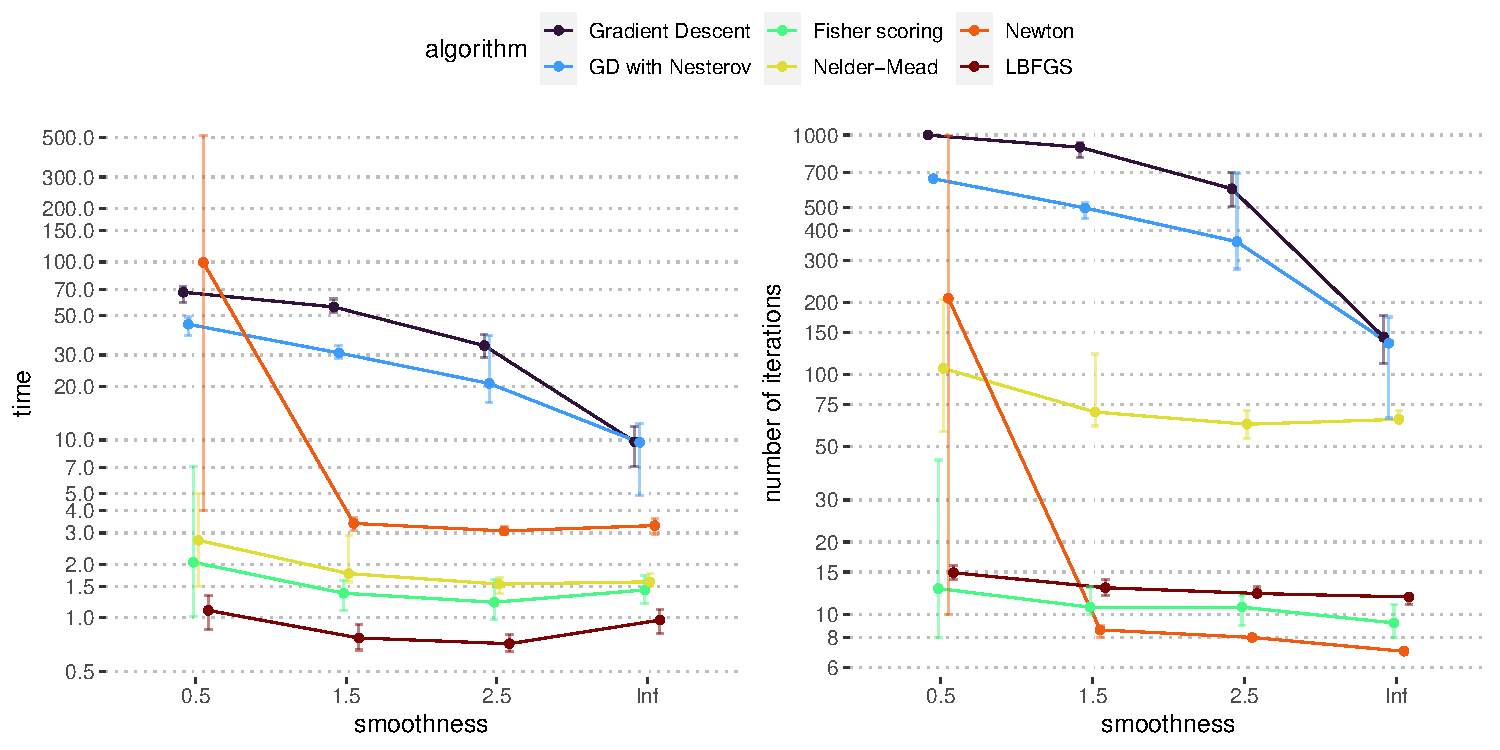
\includegraphics[width=.9\textwidth]{Borehole_comparison_0426} %<< no file extension
  %%         --- .5\textwidth stands for 50% of text width
  \caption[Times of Borehole function: line graphs with range bars]%<<-- Legend for the list of figures at the beginning of you thesis
  {Comparison of different methods using mis-specified GP models on data from Borehole function, default starting values, 10 repetitions. Y-axes are in $\log 10$ scale.}% legend displayed below the graph.
  \label{fig:plotset}
\end{figure}

\subsection{Piston function}

The 7-dimensional Piston function, which models the circular motion of a piston within a cylinder, is sampled with 1000 uniformly distributed points, and the results are displayed in Figure 3.18. The convergence check shows that when $\nu=0.5$, Newton's method fails to converge in 2 (of 10) repetitions. 

\begin{figure}[hbt!]%--- Picture 'H'ere, 'B'ottom or 'T'op; '!' 
  \centering
  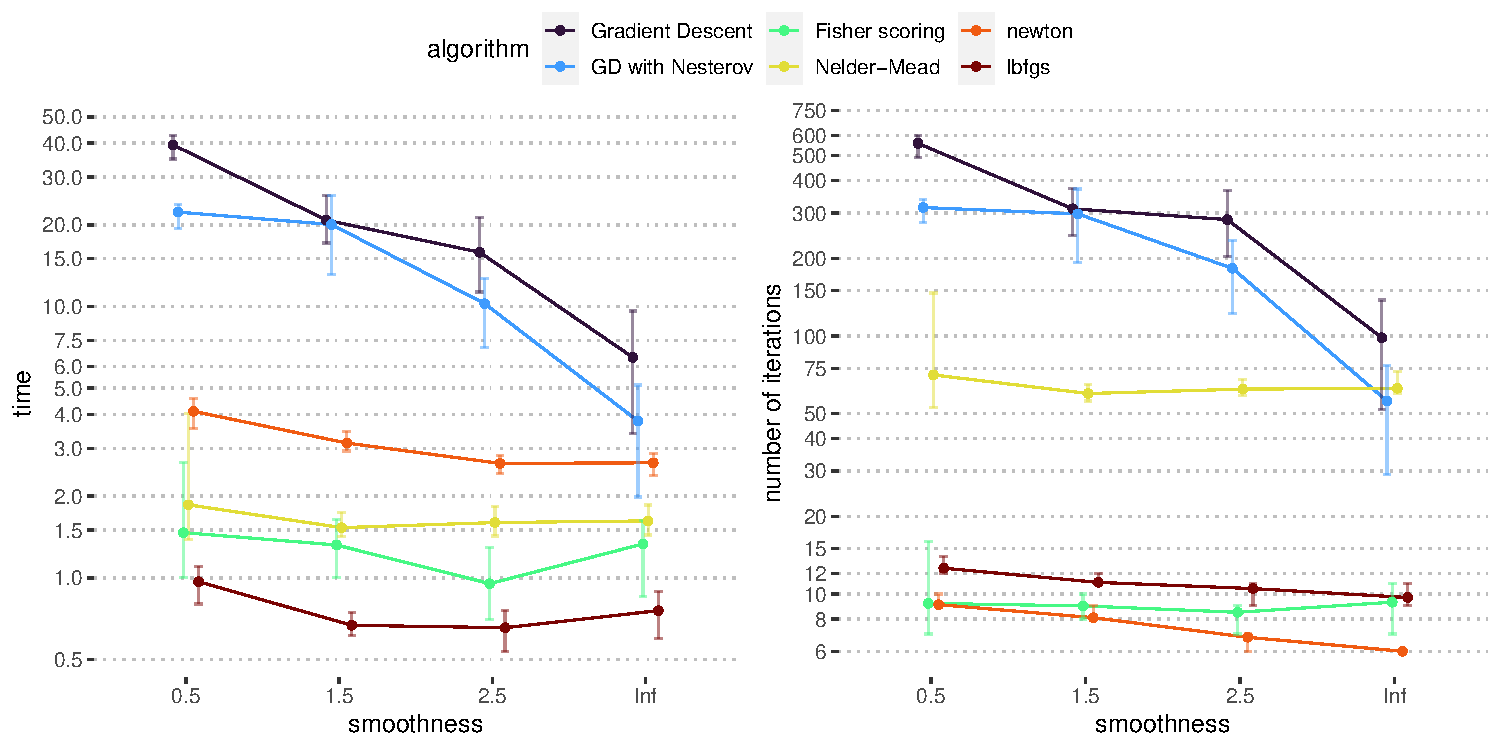
\includegraphics[width=.9\textwidth]{Piston_comparison_0426} %<< no file extension
  %%         --- .5\textwidth stands for 50% of text width
  \caption[Times of Piston function: line graphs with range bars]%<<-- Legend for the list of figures at the beginning of you thesis
  {Comparison of different methods using mis-specified GP models on data from Piston function, default starting values, 10 repetitions. Y-axes are in $\log 10$ scale.}% legend displayed below the graph.
  \label{fig:plotset}
\end{figure}

\subsection{Large scale optimization}

We want to explore the performance of optimization methods on the large scale of deterministic functions. We generate random samples of 20000 points and fit GP-Mat\'ern models with Vecchia approximation. Again, we perform the convergence check, but with stricter relative tolerance of 0.0001, since the original tolerance would not be precise enough due to the large log-likelihood values of this sample size. 

The results of Branin, Borehole, and Piston functions are displayed in Figures 3.19, 3.20 and 3.21. Among the six optimization methods, LBFGS consistently shows excellent performance of optimization for all of the three deterministic functions. 


\begin{figure}[hbt!]%--- Picture 'H'ere, 'B'ottom or 'T'op; '!' Try to
                    %impose your will to LaTeX
  \centering
  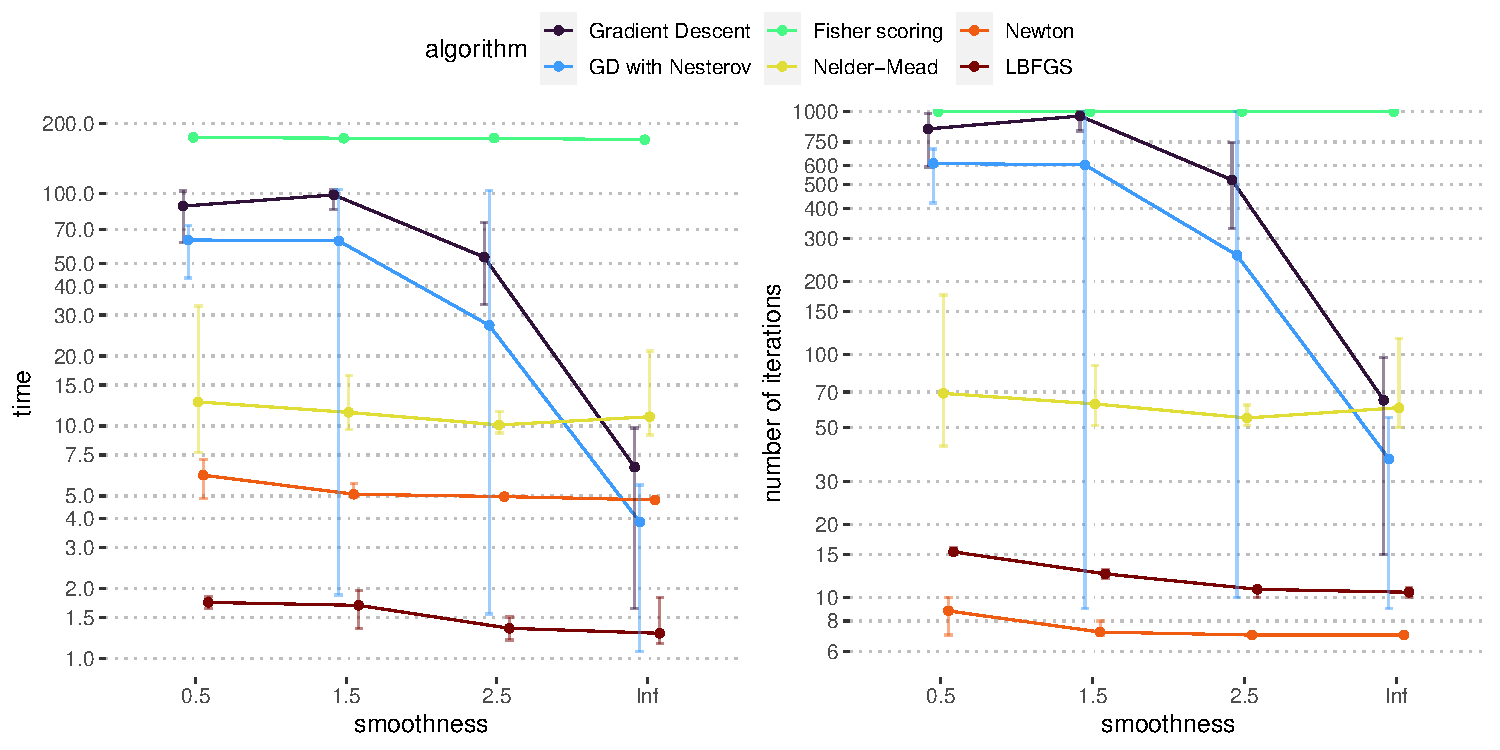
\includegraphics[width=.9\textwidth]{Branin_20000} %<< no file extension
  %%         --- .5\textwidth stands for 50% of text width
  \caption[Times of Branin of 20000 points: line graphs with range bars]%<<-- Legend for the list of figures at the beginning of you thesis
  {Comparison of different methods using GP models on 20000 points data from Branin function, default starting values, 10 repetitions. Y-axes are in $\log 10$ scale.}% legend displayed below the graph.
  \label{fig:plotset}
\end{figure}

\begin{figure}[hbt!]%--- Picture 'H'ere, 'B'ottom or 'T'op; '!' Try to
                    %impose your will to LaTeX
  \centering
  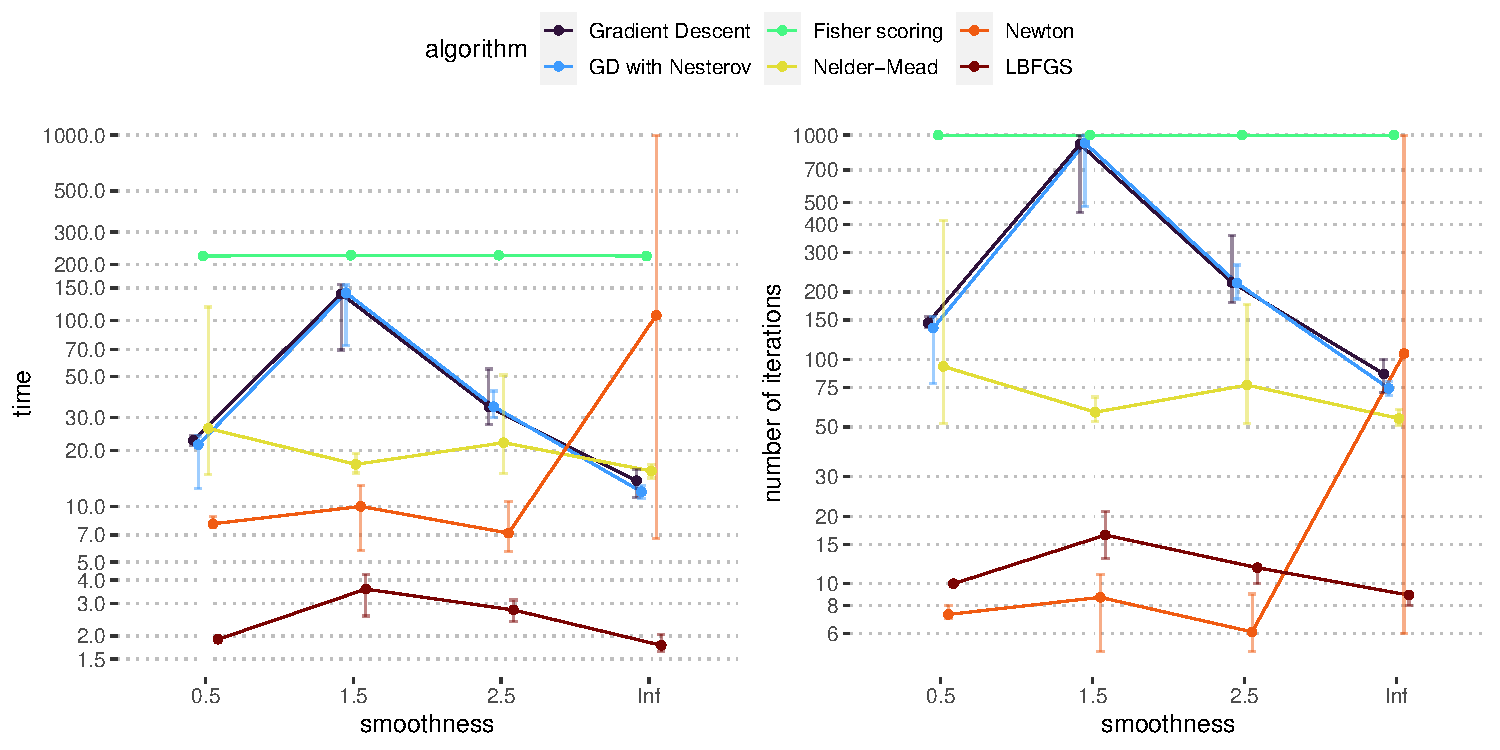
\includegraphics[width=.9\textwidth]{Borehole_20000} %<< no file extension
  %%         --- .5\textwidth stands for 50% of text width
  \caption[Times of Borehole of 20000 points: line graphs with range bars]%<<-- Legend for the list of figures at the beginning of you thesis
  {Comparison of different methods using GP models on 20000 points data from Borehole function, default starting values, 10 repetitions. Y-axes are in $\log 10$ scale.}% legend displayed below the graph.
  \label{fig:plotset}
\end{figure}

\begin{figure}[hbt!]%--- Picture 'H'ere, 'B'ottom or 'T'op; '!' Try to
                    %impose your will to LaTeX
  \centering
  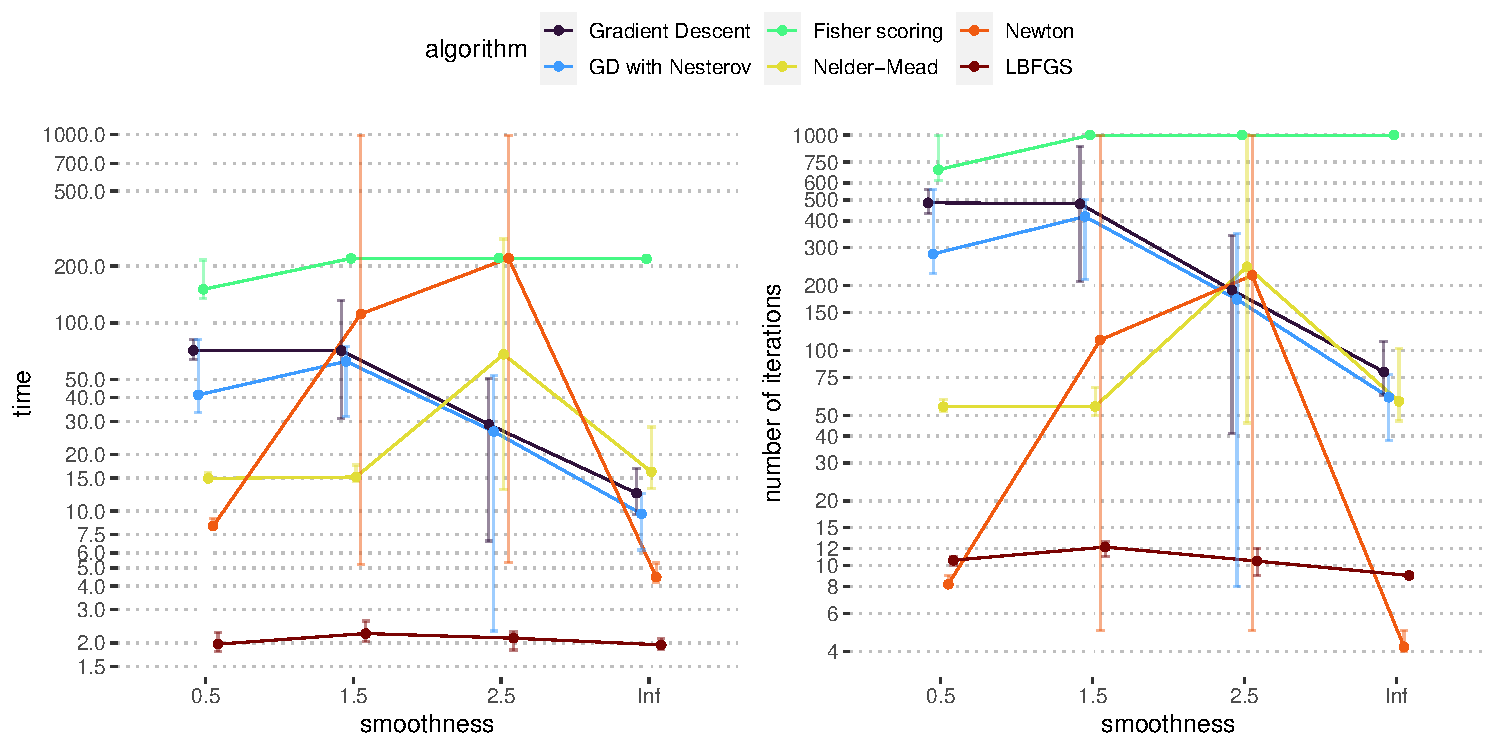
\includegraphics[width=.9\textwidth]{Piston_20000} %<< no file extension
  %%         --- .5\textwidth stands for 50% of text width
  \caption[Times of Piston of 20000 points: line graphs with range bars]%<<-- Legend for the list of figures at the beginning of you thesis
  {Comparison of different methods using GP models on 20000 points data from Piston function, default starting values, 10 repetitions. Y-axes are in $\log 10$ scale.}% legend displayed below the graph.
  \label{fig:plotset}
\end{figure}

The convergence problems of Branin large data experiment are:


\begin{itemize}
    \item With any smoothness, Fisher-scoring fails to converge within prescribed 1000 steps in any repetition.
    \item When $\nu = 1.5$, GD with Nesterov accelerator fails in 5 (of 10) repetitions.
\end{itemize}

For experiment of large data from Borehole function, the convergence check shows that:

\begin{itemize}
    \item With any smoothness, Fisher-scoring fails to converge within prescribed 1000 steps in any repetition of all smoothness settings.
    \item When $\nu = 1.5$, Newton fails in 2 (of 10) repetitions.
    \item When $\nu = 2.5$, Newton fails in 8 (of 10) repetitions.
    \item When $\nu = \inf$, Newton fails in 1 (of 10) repetition.
\end{itemize}

For experiment of large data from Piston function, the convergence check shows that:

\begin{itemize}
    \item When $\nu=0.5$, Fisher-scoring fails in 5 (of 10) repetitions.
    \item When $\nu=1.5$, 2.5, or $\infty$, Fisher-scoring fails to converge within prescribed 1000 iterations in all repetitions.
    \item When $\nu = 1.5$, Newton fails in 8 (of 10) repetitions.
    \item When $\nu = 2.5$, Newton fails in 10 (of 10) repetitions, Nelder-Mead fails in 2 (of 10) repetitions.
\end{itemize}





%%% Local Variables: 
%%% mode: latex
%%% TeX-master: "MasterThesisSfS"
%%% End: 

%%\include{Chapter...}
\chapter{Conclusions}
\label{s:Conclusions}

In this thesis, we have explored the performance of different optimization methods for Gaussian processes hyper-parameter estimation based on \texttt{GPBoost} library, taking into account the training time, for both probabilistic and deterministic functions, and in both regression and classification models. We also include two state-of-the-art approximations (Vecchia, FITC) for GP models to reduce the computational time and space complexity as large as $\mathcal{O}(n^3)$ and $\mathcal{O}(n^2)$ in large scale optimization.

As can be seen from the results, LBFGS shows an excellent and more stable performance in terms of both training speed and convergence robustness compared to the other methods. Gradient Descent shows robustness in case of mis-specification, but still risks a slower training speed and is susceptible to the shape of the log marginal likelihood. GD, Newton and Fisher-scoring can get stuck in local optima and struggle with non-convex objective functions, making them excruciatingly slow on some difficult problems. Nelder-Mead, the derivative-free method, can perform in some circumstance but unable to cope with the increasing numbers of parameters and has a higher computational cost. 

The experimental results also show that many factors, such as initialization strategy and reparameterization, affect the convergence time of the optimization methods. By choosing a reasonable starting point, the optimization methods, especially Newton's method, could perform significantly better. The \textit{log} reparameterization of the hyper-parameters $(\rho, \sigma^2_f, \sigma^2_n)$ with positive constraints could facilitate the convergence, which is also suggested in \cite{basak2021numerical}.

The choice of optimization method depends on the specific context and requirements of the application. Different optimization methods have their own advantages depending on the nature of data and the objective function. Without knowing much information about the underlying distribution, LBFGS can be a better and versatile choice for various optimization landscapes, but combining the characteristics of dataset and the computational environment is still necessary. Future research could focus on including more types of simulation data and investigating the real world dataset.





%%% Local Variables: 
%%% mode: latex
%%% TeX-master: "MasterThesisSfS"
%%% End: 
 

%%%%%%%%%%%%%%%%%%%%%%%%%%%%%%%%%%%%%%%%%%%%%%%%%
%%% Bibliography                              %%%
%%%%%%%%%%%%%%%%%%%%%%%%%%%%%%%%%%%%%%%%%%%%%%%%%
\addtocontents{toc}{\vspace{.5\baselineskip}}
\cleardoublepage
\phantomsection
\addcontentsline{toc}{chapter}{\protect\numberline{}{Bibliography}}
%\typeout{}
\bibliography{myReferences}
%% All books from our library (SfS) are already in a BiBTeX file
%% 'Assbib.bib' (included here as well), using
%\bibliography{myReferences,Assbib}
% ---------------------------------- instead of the above



%%%%%%%%%%%%%%%%%%%%%%%%%%%%%%%%%%%%%%%%%%%%%%%%% 
%%% Appendices (if needed, e.g. for R code)   %%%
%%%%%%%%%%%%%%%%%%%%%%%%%%%%%%%%%%%%%%%%%%%%%%%%%
\addtocontents{toc}{\vspace{.5\baselineskip}}
\appendix
% \include{Appendix_result1}
% \chapter{Complementary information}
\label{app:complement}

Additional material. For example long mathematical derivations could be
given in the appendix. Or you could include part of your code that is
needed in printed form. You can add several Appendices to your thesis (as
you can include several chapters in the main part of your work).

\section{Including \Rp code with verbatim}
A simple (rather too simple, see~\ref{App:listings}) way to include code or
{\it R} output is to use 
\texttt{verbatim}. It just prints the text however it is (including all
spaces, ``strange'' symbols,...) in a slightly different font.
\begin{verbatim}
## loading packages
library(RBGL)
library(Rgraphviz)
library(boot)

## global variables
X_MAX <- 150

   This allows me to put as many s  p a   c es   as I want.
I can also use \ and ` and & and all the rest that is usually only 
accepted in the math mode.

I can also make as 
                  many 
             line 
    breaks as 
I want... and
             where I want. 
\end{verbatim}

But really recommended,  much better is the following:

\section{Including \Rp code with the \emph{listings} package}\label{App:listings}
However, it is much nicer to use the \emph{listings} package to include \Rp
code in your report. It allows you to number the lines, color the comments
differently than the code, and so on.
All the following is produced by simply writing
\verb! \lstinputlisting{Pictures/picture.R} !  in your \LaTeX\ ``code'':

\lstinputlisting{Pictures/picture.R}

or \verb!\lstinputlisting{/u/maechler/R/Pkgs/sfsmisc/R/ellipse.R}! :

\lstinputlisting{ellipse.R}% was /u/maechler/R/Pkgs/sfsmisc/R/ellipse.R

\section{Using \texttt{Sweave} (or \texttt{knitr}) to include \Rp code (and more) in your report}
The easiest (and most elegant) way to include \Rp code and its output (and
have all your figures up to date with your report) is to use Sweave---or the
\href{https://cran.R-project.org/package=knitr}{\texttt{knitr}} R package with even more possibilities.
% You can find an introduction Sweave in \texttt{/u/sfs/StatSoftDoc/Sweave/Sweave-tutorial.pdf}.

Search the web to find lots of intro material on how to use Sweave or
\href{https://en.wikipedia.org/wiki/Knitr}{knitr (on Wikipedia)}.

%%% Local Variables: 
%%% mode: latex
%%% TeX-master: "MasterThesisSfS"
%%% End: 

% \include{Appendix2}
% \include{Appendix_more_R}


%% Epilogue (optional)
% \addtocontents{toc}{\vspace{.5\baselineskip}}
% \cleardoublepage
% \phantomsection
% \addcontentsline{toc}{chapter}{\protect\numberline{}{Epilogue}}
% \markboth{Epilogue}{Epilogue}
% \include{Epilogue}


%%%%%%%%%%%%%%%%%%%%%%%%%%%%%%%%%%%%%%%%%%%%%%%%%% 
%%% Declaration of originality (Do not remove!)%%%
%%%%%%%%%%%%%%%%%%%%%%%%%%%%%%%%%%%%%%%%%%%%%%%%%%
%% Instructions:
%% -------------
%% fill in the empty document confirmation-originality.pdf electronically
%% print it out and sign it
%% scan it in again and save the scan in this directory with name
%% confirmation-originality-scan.pdf 
%%
%% General info on plagiarism:
%% https://www.ethz.ch/students/en/studies/performance-assessments/plagiarism.html 
\cleardoublepage

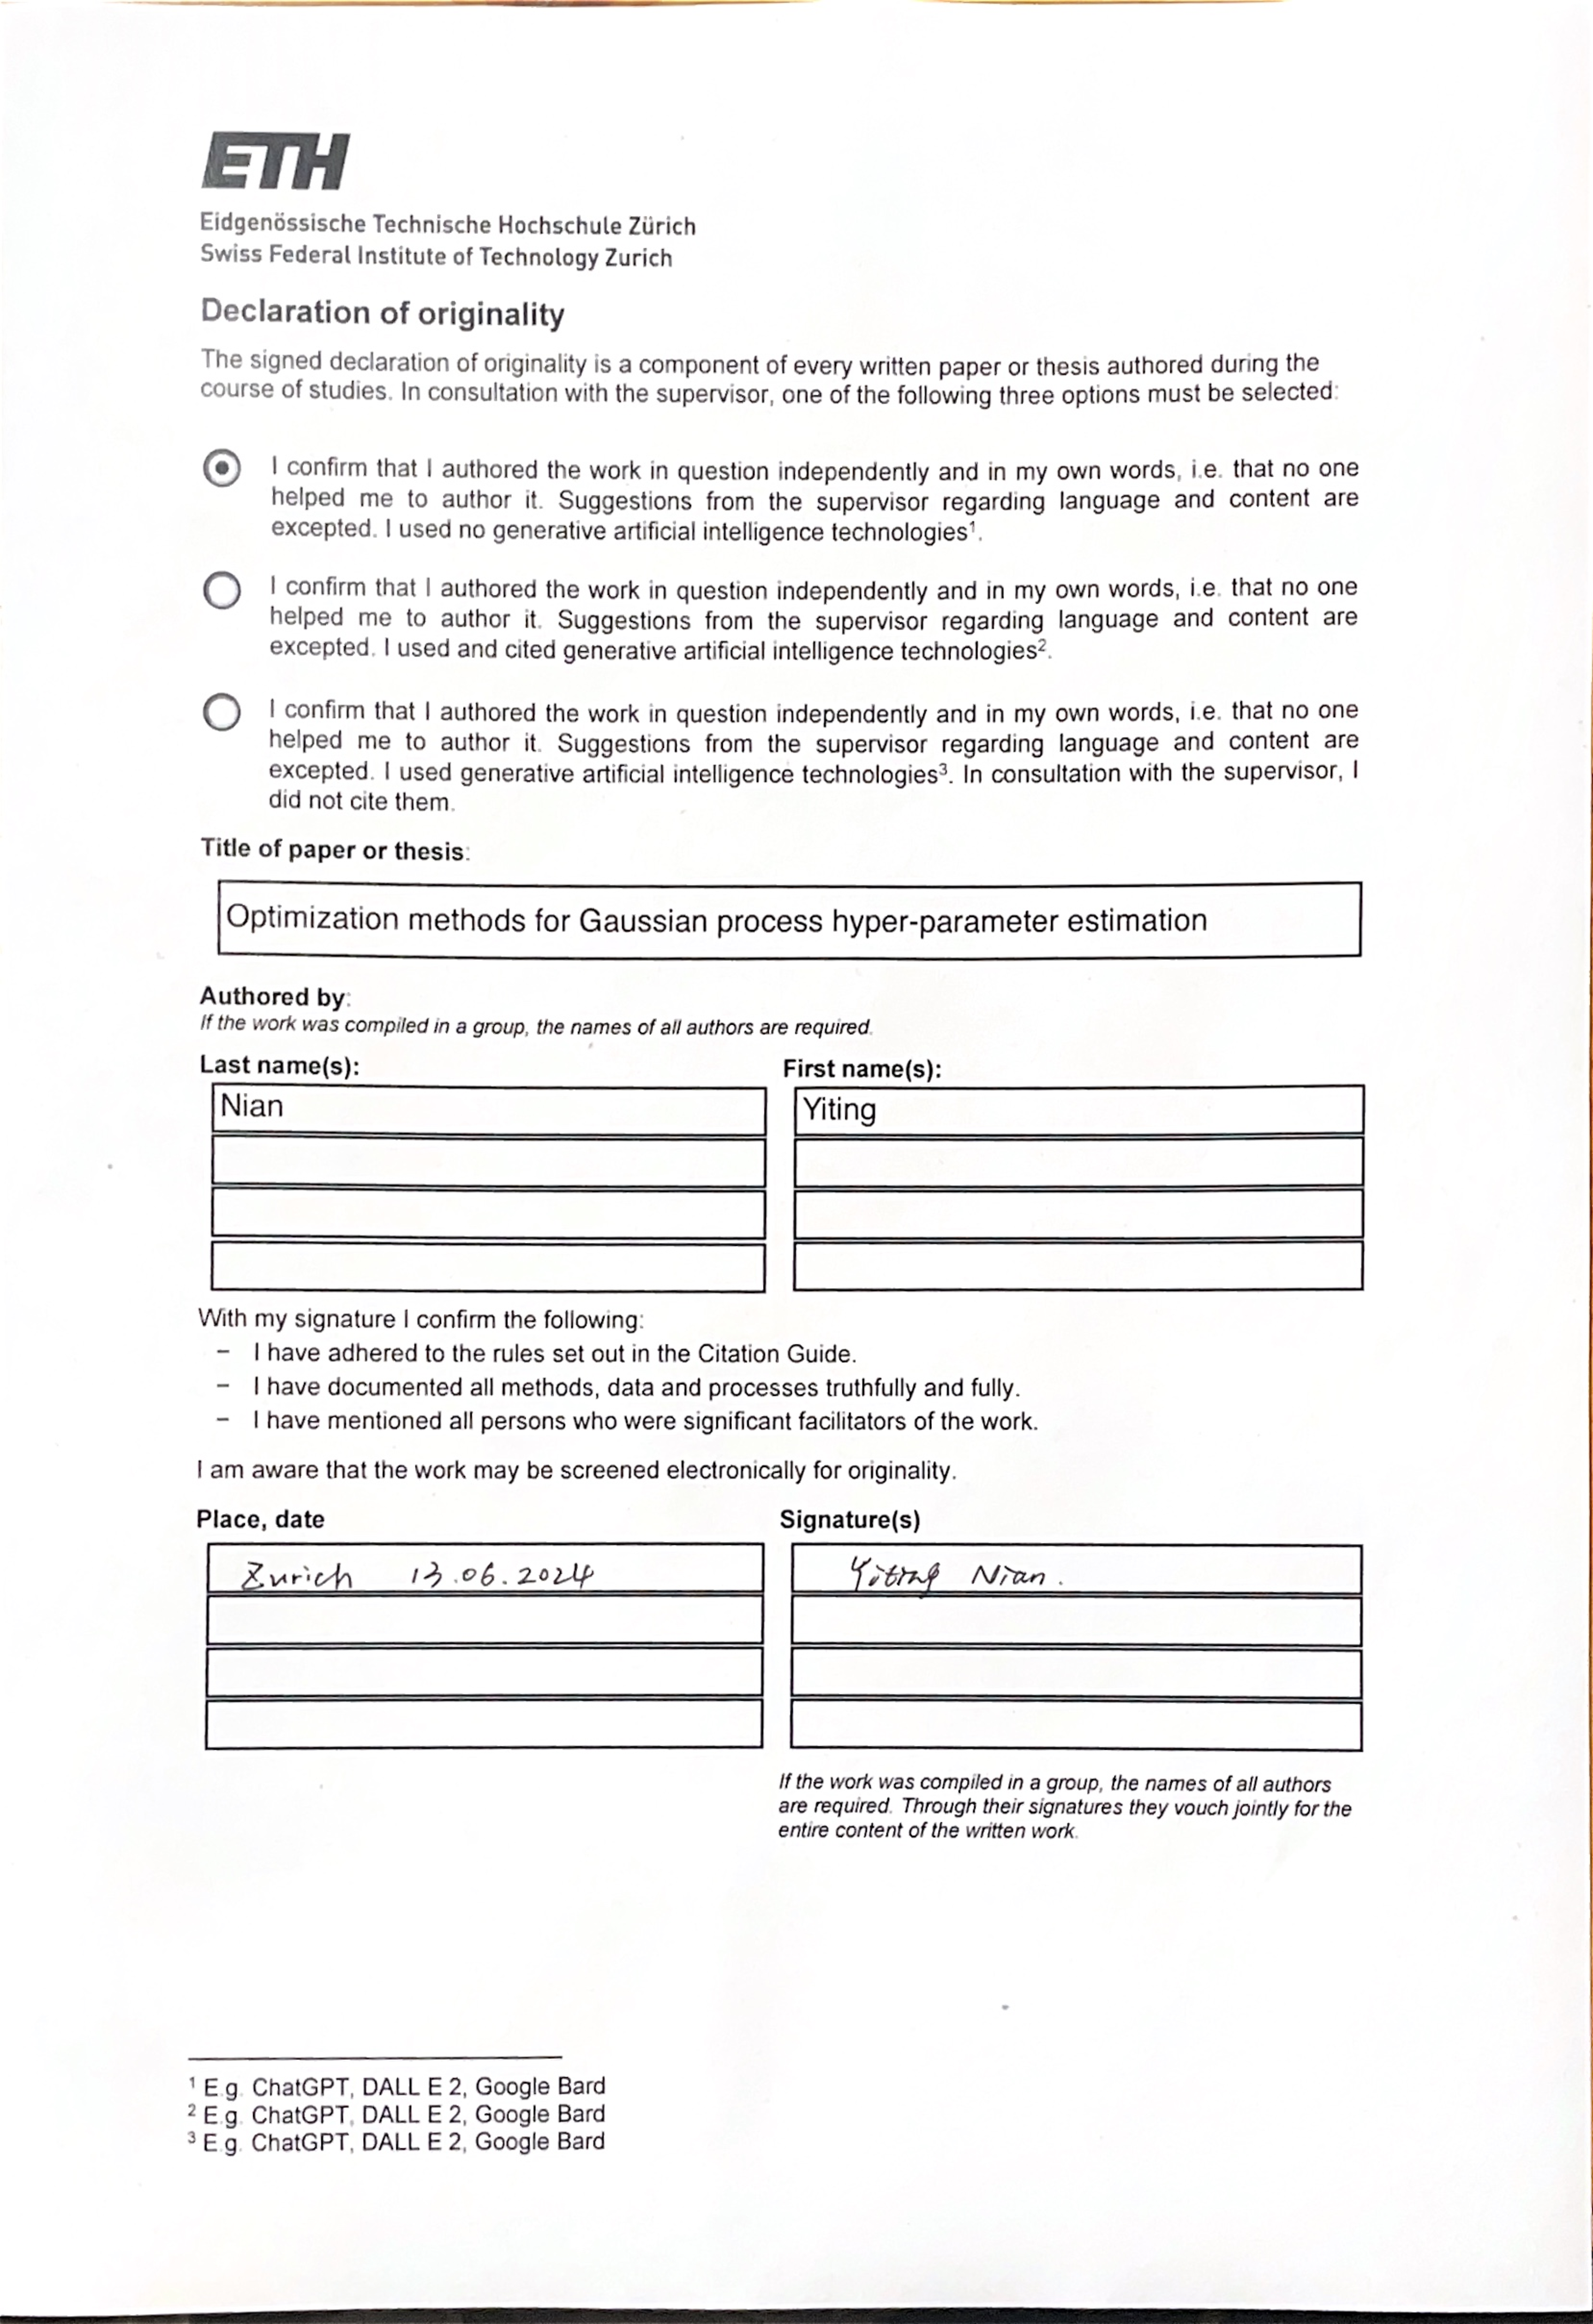
\includepdf[pages={-}, frame=true,scale=1]{confirmation-originality-scan.pdf}
\end{document}

%%% Local Variables:
%%% mode: latex
%%% TeX-master: "MasterThesisSfS"
%%% End:
